% !TEX program = xelatex
% =============================================================================
%  全国大学生数学建模竞赛（CUMCM）LaTeX 模板
%  对应 Typst 模板 zh/cumcm/main.typ 的全部功能。
%
%  字体依赖（正文宋体 / 标题黑体 / 强调楷体）：
%    - 规范字体：SimSun（宋体）、SimHei（黑体）、KaiTi（楷体）。
%    - 本模板默认使用 ctex 的 fontset=mac，在 macOS 上自动选用同族等价字体
%      Songti SC / Heiti SC / Kaiti SC，确保开箱即用。
%    - 若系统已安装 SimSun/SimHei/KaiTi（如 Windows 或手动安装），可将下方
%      \documentclass 选项 fontset=mac 改为 fontset=windows，即可使用规范字体。
%    - 西文正文：Times New Roman；代码等宽：Menlo（缺失时回退到默认字体）。
%  编译方式：xelatex main.tex （需运行两遍以生成目录）
% =============================================================================
\documentclass[fontset=windows, 12pt, a4paper]{ctexart}

% ---------- 页面：A4，上下左右 2.5cm ----------
\usepackage[a4paper, top=2.5cm, bottom=2.5cm, left=2.5cm, right=2.5cm]{geometry}

% ---------- 数学 ----------
\usepackage{amsmath}
\usepackage{amssymb}
\usepackage{graphicx}
\usepackage{float}
\usepackage{tikz}
\usetikzlibrary{arrows.meta, positioning}

% ---------- 图注：小一号字、更小间距 ----------
\usepackage{caption}
\captionsetup{font=small, skip=4pt}

% ---------- 浮动体控制：每页至多一张图，章末强制清空浮动队列 ----------
\usepackage{placeins}
\usepackage{needspace}
\AtBeginDocument{%
  \setcounter{topnumber}{1}%
  \setcounter{bottomnumber}{0}%
  \setcounter{totalnumber}{1}%
  \renewcommand{\topfraction}{0.95}%
  \renewcommand{\bottomfraction}{0.9}%
  \renewcommand{\textfraction}{0.05}%
  \renewcommand{\floatpagefraction}{0.95}%
}

% ---------- 字体（fontspec + ctex，xelatex 编译） ----------
% 中文宋体/黑体/楷体由 ctex 的 fontset=mac 自动设置（Songti SC / Heiti SC / Kaiti SC），
% 并自动定义 \songti / \heiti / \kaishu 等字体命令。
% 西文正文与代码等宽字体：
\IfFontExistsTF{Times New Roman}{\setmainfont{Times New Roman}}{}
\IfFontExistsTF{Menlo}{\setmonofont{Menlo}}{}

% ---------- 正文：12pt，首行缩进 2em，两端对齐，行距约 1.38 倍 ----------
% \linespread{1.13} 对应行高约 1.36 倍字号
\linespread{1.13}
\setlength{\parindent}{2em}
\setlength{\emergencystretch}{2em}

% ---------- 公式上下间距收紧（不影响可读性） ----------
\AtBeginDocument{%
  \setlength{\abovedisplayskip}{4pt plus 2pt minus 2pt}%
  \setlength{\belowdisplayskip}{4pt plus 2pt minus 2pt}%
  \setlength{\abovedisplayshortskip}{2pt plus 2pt}%
  \setlength{\belowdisplayshortskip}{3pt plus 2pt minus 2pt}%
}

% ---------- 标题编号（\ctexset 配置） ----------
% 一级标题用中文数字“一、二、三、”，二级及以下用 1.1 / 1.1.1
\ctexset{
  section/number       = \chinese{section},
  subsection/number    = \arabic{section}.\arabic{subsection},
  subsubsection/number = \arabic{section}.\arabic{subsection}.\arabic{subsubsection},
}

% ---------- 标题格式（titlesec 配置） ----------
\usepackage{titlesec}
\titleformat{\section}
  {\centering\fontsize{17.3pt}{20.8pt}\heiti\bfseries}
  {\chinese{section}、}{1em}{}
\titleformat{\subsection}
  {\fontsize{14.45pt}{17.4pt}\heiti\bfseries}
  {\arabic{section}.\arabic{subsection}}{1em}{}
\titleformat{\subsubsection}
  {\fontsize{12.05pt}{14.5pt}\heiti\bfseries}
  {\arabic{section}.\arabic{subsection}.\arabic{subsubsection}}{1em}{}
\titlespacing{\section}       {0pt}{1.0em}{0.6em}
\titlespacing{\subsection}    {0pt}{0.85em}{0.4em}
\titlespacing{\subsubsection} {0pt}{0.85em}{0.4em}

% ---------- 目录（tocloft 点线引导） ----------
\usepackage{tocloft}
\renewcommand{\cftsecfont}{\heiti\bfseries}
\renewcommand{\cftsecpagefont}{\heiti\bfseries}
\renewcommand{\cftsecleader}{\cftdotfill{\cftdotsep}}
\renewcommand{\cftsubsecleader}{\cftdotfill{\cftdotsep}}
\renewcommand{\cftsubsubsecleader}{\cftdotfill{\cftdotsep}}

% ---------- 表格与代码 ----------
\usepackage{booktabs}
\usepackage{array}
\usepackage{longtable}
\usepackage{xcolor}
\usepackage{listings}
\lstset{
  basicstyle=\ttfamily\small,
  backgroundcolor=\color{black!3},
  frame=single,
  framesep=6pt,
  xleftmargin=8pt,
  xrightmargin=8pt,
  rulecolor=\color{black!30},
  framerule=0.8pt,
  breaklines=true,
  showstringspaces=false,
  columns=fullflexible,
  keepspaces=true,
}

% ---------- 页码：底部居中 ----------
\pagestyle{plain}

% ---------- 自定义命令（对应 Typst 函数） ----------
% \papertitle{标题}：居中 17.3pt 加粗标题
\newcommand{\papertitle}[1]{%
  \thispagestyle{empty}%
  \begin{center}
    {\fontsize{17.3pt}{22pt}\bfseries #1}
  \end{center}
  \vspace{1em}
}
% \abstractcn{摘要正文}{关键词}：居中“摘要”标题（14pt 加粗）+ 正文 + “关键字：”加粗 + 关键词 + 换页
\newcommand{\abstractcn}[2]{%
  \thispagestyle{empty}%
  {\centering {\fontsize{14pt}{17pt}\bfseries 摘要}\par}%
  \vspace{0.4em}%
  #1\par
  \vspace{0.6em}%
  {\heiti\bfseries 关键字：}#2\par
  \newpage
}
% \tocpage：目录页，标题“目录”居中 17.3pt 黑体加粗，点线引导
\makeatletter
\newcommand{\tocpage}{%
  \setcounter{page}{1}%
  \begin{center}
    {\fontsize{17.3pt}{20.8pt}\heiti\bfseries 目录}
  \end{center}
  \vspace{0.5em}
  \@starttoc{toc}%
  \newpage
}
\makeatother
% \referencescn：参考文献节，标题“参考文献”（不带编号但进目录）
\newcommand{\referencescn}{%
  \addcontentsline{toc}{section}{参考文献}%
  % 参考文献。注意：main.tex 中 \referencescn 已通过 thebibliography 自动生成
% “参考文献”一级标题（不带编号），并已 \addcontentsline 进入目录，
% 所以本文件**不要再写一级标题**，否则会出现两个“参考文献”标题。

\begin{thebibliography}{99}
\small
\setlength{\itemsep}{0pt}\setlength{\parsep}{0pt}\setlength{\parskip}{0pt}%
\bibitem{ref1} 姜启源, 谢金星, 叶俊. 数学模型[M]. 5 版. 北京: 高等教育出版社, 2018.
\bibitem{ref2} 司守奎, 孙玺菁. 数学建模算法与应用[M]. 3 版. 北京: 国防工业出版社, 2021.
\bibitem{ref3} Birge J R, Louveaux F. Introduction to Stochastic Programming[M]. 2nd ed. New York: Springer, 2011.
\bibitem{ref4} Hyndman R J, Athanasopoulos G. Forecasting: Principles and Practice[M]. 3rd ed. Melbourne: OTexts, 2021.
\bibitem{ref7} Hoerl A E, Kennard R W. Ridge regression: biased estimation for nonorthogonal problems[J]. Technometrics, 1970, 12(1): 55-67.
\end{thebibliography}
%
}
% \appendixcn：附录节，标题“附录 A  核心代码”
\newcommand{\appendixcn}{%
  \section*{附录 A\quad 核心代码}%
  \addcontentsline{toc}{section}{附录 A\quad 核心代码}%
  \vspace{1.1em}

本节给出各问题求解程序的核心代码片段，完整程序见随论文提交的源码文件。

\vspace{0.6em}
{\heiti\bfseries （1）问题一：电力平衡、储能递推与充放电互斥约束构建}

\begin{lstlisting}[language=Python]
N, DT, SOC_MIN, SOC_MAX = 144, 1/6, 1200.0, 10800.0
SOC_INITIAL = SOC_TERMINAL = 6000.0
ENERGY_MAX = 5000.0 * DT          # 833.333333 kWh
ETA_C = ETA_D = 0.9

# variables: purchase | charge | discharge | soc | curtailment ( | mode )
# power balance: G - C + D - W = L - P
for t in range(N):
    for col, val in [(purchase[t], 1.0), (charge[t], -1.0),
                     (discharge[t], 1.0), (curtailment[t], -1.0)]:
        add_eq(row, col, val)
    rhs.append(load_kwh[t] - pv_kwh[t])

# storage recursion: B_t - B_{t-1} - eta_c*C_t + D_t/eta_d = 0
for t in range(N):
    terms = [(soc[t], 1.0), (charge[t], -ETA_C), (discharge[t], 1.0/ETA_D)]
    if t > 0:
        terms.append((soc[t-1], -1.0))
    for col, val in terms:
        add_eq(row, col, val)
    rhs.append(SOC_INITIAL if t == 0 else 0.0)

# terminal condition B_144 = B_0
add_eq(row, soc[-1], 1.0); rhs.append(SOC_TERMINAL)

# MILP only: mutual exclusion C_t <= Emax*z_t, D_t <= Emax*(1-z_t)
for t in range(N):
    add_ub(charge[t], 1.0);  add_ub(mode[t], -ENERGY_MAX); ub.append(0.0)
    add_ub(discharge[t], 1.0); add_ub(mode[t], ENERGY_MAX); ub.append(ENERGY_MAX)

objective = np.zeros(nvar); objective[purchase] = price
integrality = np.zeros(nvar, dtype=int); integrality[mode] = 1
result = milp(objective, integrality=integrality, bounds=Bounds(lower, upper),
              constraints=[LinearConstraint(a_eq, b_eq, b_eq),
                           LinearConstraint(a_ub, -np.inf, ub)],
              options={"mip_rel_gap": 0.0, "presolve": True})
\end{lstlisting}

\vspace{0.6em}
{\heiti\bfseries （2）问题二：周期加权预测与整日联合残差场景}

\begin{lstlisting}[language=Python]
RHO = 0.8

def exponential_weights(k):
    w = RHO ** np.arange(k, dtype=float)
    return w / w.sum()

# load: last min(4, floor((d-1)/7)) same-weekday samples
k = min(4, (day - 1) // 7)
indices = day - 7 * np.arange(1, k + 1)
load_hat = np.maximum(np.average(load[indices], axis=0,
                                 weights=exponential_weights(k)), 0.0)

# joint residual sampling: whole 144-step daily blocks, same historical date
omega = 0.98 ** (day - r) * (1.0 + (weekday[day] == weekday[r]))
prob = omega / omega.sum()
chosen = rng.choice(len(history), size=S, p=prob)      # S = 100
load_scen = np.maximum(load_hat[None, :] + resid_L[chosen], 0.0)
pv_scen = np.minimum(pv_max_observed,
                     np.maximum(pv_hat[None, :] + resid_P[chosen], 0.0))
\end{lstlisting}

\vspace{0.6em}
{\heiti\bfseries （3）问题二：季节余弦终端软区间与因果风险微调}

\begin{lstlisting}[language=Python]
SOC_BASE, SOC_AMP, PHASE_DAY = 7000.0, 800.0, 15.0
BAND_HALF, RISK_GAIN, RISK_CAP = 1000.0, 200.0, 600.0
RISK_WINDOW, RISK_FLOOR = 56, 100.0

def seasonal_reference(date):
    return SOC_BASE + SOC_AMP * np.cos(
        2.0 * np.pi * (date.dayofyear - PHASE_DAY) / 365.0)

# risk score: 80th percentile minus mean of the daily net-load scenario total
score = np.quantile(net_total, 0.80) - net_total.mean()

# causal window: only days strictly before the current decision day
hist = scores[max(0, day - RISK_WINDOW):day]
median = float(np.median(hist))
scale = max(1.4826 * np.median(np.abs(hist - median)), RISK_FLOOR)
adj = np.clip(RISK_GAIN * (score - median) / scale, -RISK_CAP, RISK_CAP)

ref = float(np.clip(seasonal_reference(date) + adj, 5200.0, 8600.0))
lower, upper = ref - BAND_HALF, ref + BAND_HALF    # double-sided soft band
\end{lstlisting}

\vspace{0.6em}
{\heiti\bfseries （4）问题三：日内滚动调整的调整恒等式、目标函数与缺口不等式}

\begin{lstlisting}[language=Python]
# adjustment identity A_t - G_t = U_t - V_t  (net settlement)
for t in range(T):
    for col, val in [(purchase[t], 1.0), (upward[t], -1.0), (downward[t], 1.0)]:
        add_eq(row, col, val)
    rhs.append(original_plan[t])

# rolling objective on the remaining horizon
objective[upward]   =  1.5 * expected_price
objective[downward] = -0.5 * expected_price
for s in range(S):
    objective[emergency[s]] = prob[s] * 5.0 * price_scenarios[s]
objective[reserve] = RESERVE_PENALTY            # 1.1250 yuan/kWh, both bands

# scenario deficit H >= L - P + C - D - A; surplus W is recovered afterwards
# by its positive part, which keeps the feasible region unchanged.
for s in range(S):
    for t in range(T):
        add_ub(purchase[t], -1.0); add_ub(emergency[s, t], -1.0)
        add_ub(discharge[t], -1.0); add_ub(charge[t], 1.0)
        ub.append(-(load_scen[s, t] - pv_scen[s, t]))
\end{lstlisting}

\vspace{0.6em}
{\heiti\bfseries （5）问题四：固定指数周期电价预测与因果门控残差更新}

\begin{lstlisting}[language=Python]
AR_LAGS = [1, 2, 3, 6, 12, 18, 36, 72, 144]
ALPHA_GRID = [0.1, 1, 10, 20, 50, 100]

def causal_day_ahead_forecast(actual):
    forecast = np.full_like(actual, np.nan)
    for day in range(1, min(7, len(actual))):
        forecast[day] = actual[day - 1]           # warm-up only
    for day in range(7, len(actual)):
        k = min(4, day // 7)
        w = exponential_weights(k)
        idx = day - 7 * np.arange(1, k + 1)
        forecast[day] = np.maximum(np.average(actual[idx], axis=0, weights=w), 0.0)
    return forecast

# monthly causal gate: enable ridge residual update only on validated issue hours
for month in range(2, 13):
    cutoff = first_day_of_month[month]
    for i, issue_hour in enumerate([6, 12, 18], start=1):
        valid = np.arange(max(7, cutoff - 7), cutoff)
        gate_model, _ = fit_causal_ridge(flat, valid[0] * N)
        base_mae, update_mae = evaluate_on(valid, base, gate_model, start=issue_hour*6)
        use_update = update_mae < base_mae
        model, alpha = fit_causal_ridge(flat, cutoff * N)
        if use_update:
            issue_forecast[month_days, i, start:] = periodic_base + residual_hat
\end{lstlisting}\endinput
%
}
% \threelinetable{标题}{列定义}{表头}{表格内容}：三线表，标题在表格上方居中 10.5pt 黑体加粗
% 调用示例：\threelinetable{表 1 示例}{ccc}{A & B & C}{1 & 2 & 3 \\ 4 & 5 & 6}
\newcommand{\threelinetable}[4]{%
  \par\smallskip
  \begingroup
    \centering
    \setlength{\tabcolsep}{3pt}%
    {\fontsize{10.5pt}{12.6pt}\heiti\bfseries #1}\par
    \vspace{0.25em}
    \begin{tabular*}{\textwidth}{@{\extracolsep{\fill}}#2@{}}
      \toprule
      #3 \\
      \midrule
      #4 \\
      \bottomrule
    \end{tabular*}
    \par
  \endgroup
  \vspace{0.25em}
}

\begin{document}

% 封面（不编号）
\papertitle{基于周期加权预测与场景混合整数规划的微网调度策略}

% 摘要页（不编号）
\abstractcn{%
微网可在电价低谷充电、高峰放电，在满足小区负载的前提下降低购电费用。本文针对信息逐步丰富的四类场景，建立以电力平衡和储能状态递推为内核、以\textbf{混合整数线性规划}为工具的\textbf{购电与储能调度模型}。模型由完全信息下的确定性基准，依次扩展至日前不确定性、光伏预报驱动的日内滚动，以及实时波动电价下的联合更新；为维持跨日储能价值，构造随季节变化并由场景风险因果调整的\textbf{终端软区间机制}。

针对问题一，在电价、负载和光伏全部已知的\textbf{指定日}建立确定性优化模型，并以 0--1 状态变量核验充放电互斥。单日购电费用为\textbf{35126.95 元}，较无储能基准节省\textbf{26.90\%}，弃光量由 6247.96 kWh 降为 0。

针对问题二，在每日 0:00 严格使用历史信息，采用\textbf{周期加权预测、整日联合残差场景与季节终端软区间}制定日前计划：负荷取最近 4 个同星期、光伏取最近 7 日的指数加权平均（$\rho=0.8$），从已结算样本外残差中抽取 100 个完整日场景；日末储电量的季节基准在 6200$\sim$7800 kWh 间变化，并按场景净负荷风险的 80\% 分位数相对历史中位数的偏离因果调整，形成 $\pm1000$ kWh 的软区间。负荷与光伏预测的 WAPE 分别为 3.89\% 和 6.30\%。在 334 天回测期内，\textbf{实际总费用为 14637169.37 元}，较不设终端约束的方案节省 14472.01 元。

针对问题三，引入附件 3 的官方光伏预报并建立\textbf{四时点滚动模型}，按调整结算规则更新剩余时域决策。334 天的\textbf{全年总费用为 14510355.99 元}，较仅 0:00 决策节省\textbf{351055.72 元（2.36\%）}，紧急购电量减少 25.40\%；其中 6:00 和 12:00 更新贡献主要收益，18:00 的边际价值较低。

针对问题四，实时波动电价的自相关在整周滞后处形成局部峰值（第 7 个整日滞后为 0.9576）；据此以最近 4 个同星期、同时刻价格的固定指数加权模型预测电价（WAPE 6.17\%、日内 Spearman 0.9526），并用\textbf{因果门控的岭回归残差模型}进行日内更新。问题 4-2 与 4-3 的全年总费用分别为 15529514.78 元与\textbf{15393286.54 元}，后者较仅 0:00 决策节省\textbf{384819.53 元（2.44\%）}。在保持负荷、光伏信息结构及储能约束不变、仅放开未来电价的价格完全信息下界下，现实策略的\textbf{费用差距仅为 1.03\%}。

敏感性分析表明，\textbf{终端机制、场景规模和周期权重}的合理扰动不改变日内滚动调度的主要经济结论。\textbf{综上，本文策略可在不同信息条件下实现可执行且稳健的购电费用优化。}%
}{%
微网调度 \quad 混合整数线性规划 \quad 整日联合残差场景 \quad 滚动时域 \quad 周期加权预测 \quad 因果门控更新%
}

% 不设目录页，正文页码从 1 开始
\setcounter{page}{1}

\section{问题重述与问题分析}

\subsection{问题背景}

微网是一种可就地消纳分布式光伏、减少并网冲击的小型发用电系统。与外部电网并网运行时，其核心经济行为是``低买高卖''：在外网电价较低或光伏出力富余时为储能设备充电，在电价较高时放电供电，从而在满足小区负载的前提下压低购电费用。

题目数据构成一条逐层放开的``信息链''：附件 1 给出单日的电价、小区负载与光伏预测功率，附件 2 至附件 4 分别给出全年的负载与光伏实测值、四个发布时点的光伏预报、全年实时电价，附件 5 为结果填报模板。储能设备的物理边界为：容量上限 12000 kWh、最大充放电功率 5000 kW、运行区间 1200$\sim$10800 kWh、充放电效率各 90\%，2025 年 1 月 1 日 0:00 的初始储电量为 6000 kWh。二者构成四问共用的输入与约束。

\subsection{问题提出}

四问共享同一物理场景与同一套储能边界，差别只在三点：决策时点能获得哪些信息、决策变量有多少自由度、以及费用如何结算。按这一理解，四问的建模任务可概括如下。

\textbf{问题一（确定性单日调度）：}电价、负载与光伏预测全部已知，需要在日初一次性给出全天的计划购电量与充放电轨迹，使全天购电费用最小，并满足逐时段电力平衡与日初、日末储电量相等的要求。该问本质上是一个以购电费为目标、以储电量为唯一耦合变量的确定性线性规划，为后续各问提供调度内核与费用基准。

\textbf{问题二（负荷与光伏不确定下的日前决策）：}电价规律仍已知，但负载与光伏在日初尚未揭晓，只能使用此前的历史实测值；计划量一旦定下不得更改，实际出现缺口时只能以 5 倍电价紧急购电。因此该问是含预测误差的随机优化：需要分别预测当天 144 个时段的负荷与光伏，用预测误差的分布刻画不确定性，并把跨日储电量的价值写进单日模型，防止模型逐日透支储能。

\textbf{问题三（光伏预报更新下的日内滚动决策）：}在问题二的基础上，日初之外还可获得 6:00、12:00、18:00 三次更新的未来光伏预报，允许修改尚未执行时段的购电计划；上调与下调分别按 1.5 倍与 50\% 电价结算。该问由``一次决策''变为``多次滚动决策''，需要处理已执行时段的不可回溯性、剩余时域的重新优化以及调整费用的线性化，并回答引入哪些时点的预报才值得。

\textbf{问题四（波动电价下的重算）：}把固定的日内电价换成逐日变化的实时电价，要求在电价同样只能预测的前提下重算问题二与问题三，并区分``可实施的现实策略''与``假想全知的价格完全信息基准''，以量化价格预测误差造成的经济损失。

\subsection{问题分析}

四问的关系是``同一内核、逐层加难''，因此本文不为每一问另写一套模型，而是先抽出公共调度内核——逐时段电力平衡、储能状态递推、充放电互斥与储电量边界——再逐问叠加预测、场景、滚动与价格波动，形成统一的``预测---场景---优化---结算''框架。

其中，贯穿全文各类调度场景的电力平衡关系为

\begin{equation}
  P(t) + G(t) + H(t) + D(t) = L(t) + C(t) + W(t).
  \label{eq:unified_power_balance}
\end{equation}

式中，光伏可利用电量 $P(t)$、计划购电量 $G(t)$、紧急购电量 $H(t)$ 与储能放电量 $D(t)$ 共同构成时段供给；负荷电量 $L(t)$、储能充电量 $C(t)$ 与弃光（或无法消纳的富余）电量 $W(t)$ 共同构成时段去向。问题一中不发生紧急购电，故 $H(t)=0$；问题三、问题四的滚动重优化中，以调整后购电量 $A^{(\tau)}(t)$ 替代 $G(t)$。因此，各问虽在信息边界和购电机制上不同，均可由式~\eqref{eq:unified_power_balance} 保证逐时段电量守恒，关系如图~\ref{fig:unified_power_balance} 所示。

\begin{figure}[H]
  \centering
  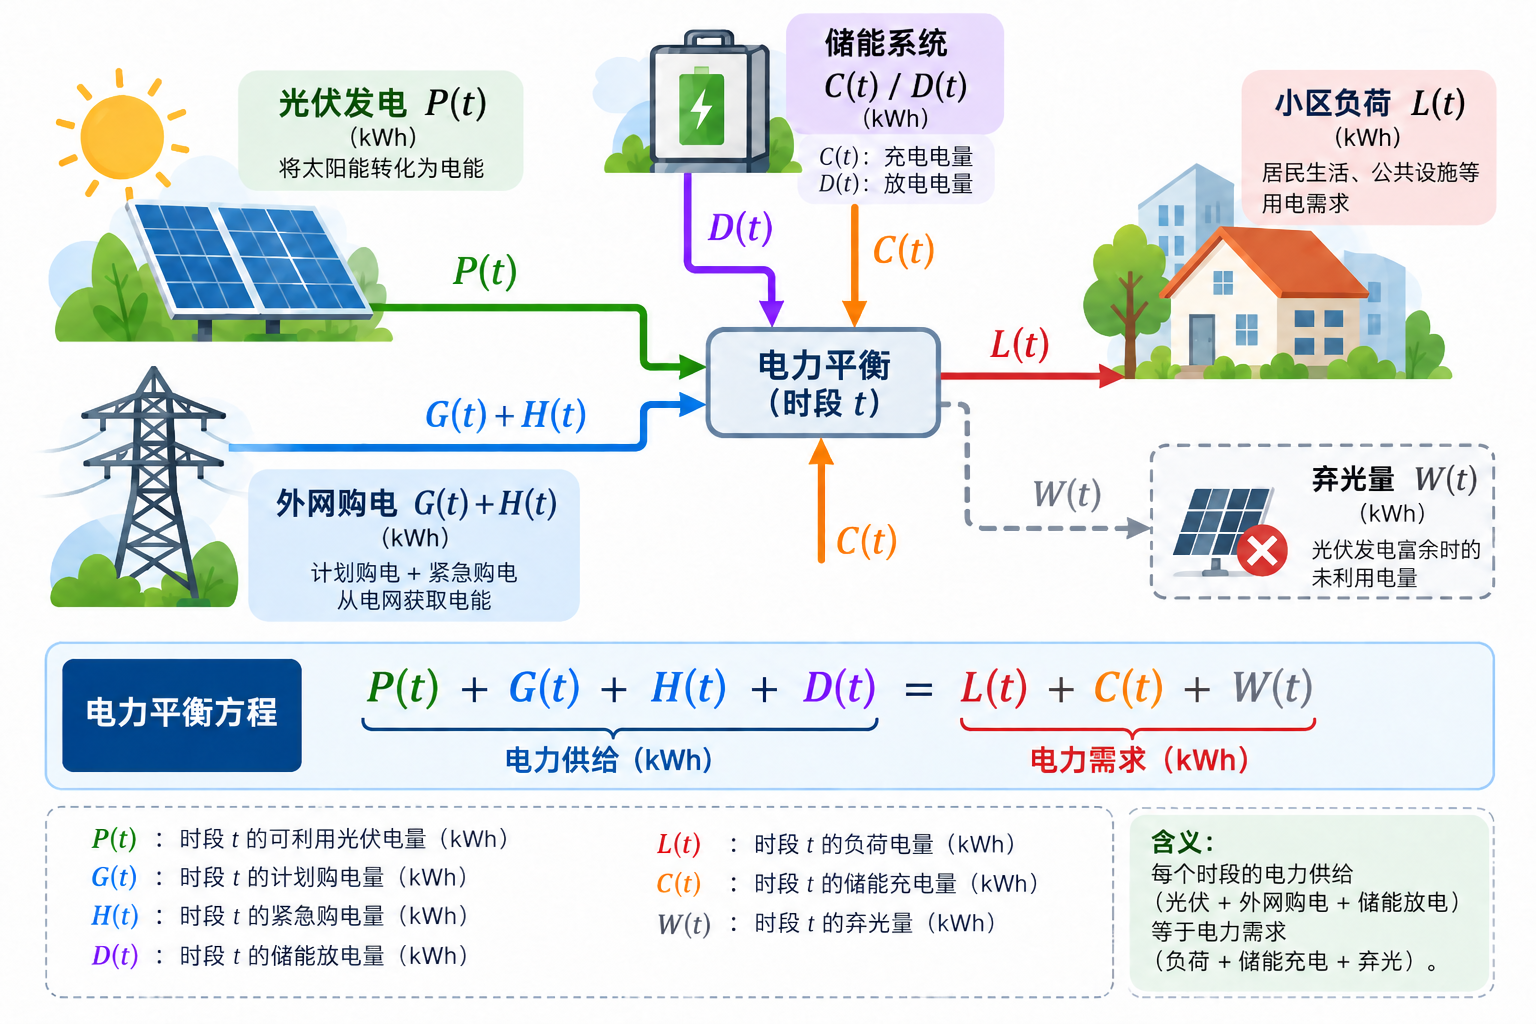
\includegraphics[width=0.96\textwidth]{../figures/电力平衡.png}
  \caption{贯穿全文的微网电力平衡关系}
  \label{fig:unified_power_balance}
\end{figure}

建模前需先锁定几处口径：10 分钟时刻标签是区间起点还是终点、90\% 是单程效率还是往返效率、问题三下调购电如何结算、问题四是否允许提前知道全天电价。这些口径直接决定结果的含义，本文在模型假设中逐条锁定基准并说明备选解释的影响，在对应小问内再结合模型交代其作用。总体技术路线如图~\ref{fig:roadmap} 所示：读取数据并统一量纲，建立公共调度内核，按各问特点扩展预测、场景或滚动机制，最后用当天实际值回放结算并校验。这样既保证模型结构一致，也便于把费用的变化归因到具体因素。

\begin{figure}[H]
  \centering
  \definecolor{cLvData}{HTML}{4A7BA7}%
  \definecolor{cLvCore}{HTML}{4C9279}%
  \definecolor{cLvSub}{HTML}{C08B45}%
  \definecolor{cLvChk}{HTML}{7E6BA8}%
  \resizebox{\textwidth}{!}{%
  \begin{tikzpicture}[
    font=\small,
    blk/.style={draw, rounded corners=2.5pt, align=center, inner sep=5pt,
                minimum height=9mm, line width=0.6pt},
    lv1/.style={blk, draw=cLvData, fill=cLvData!10},
    lv2/.style={blk, draw=cLvCore, fill=cLvCore!10},
    lv3/.style={blk, draw=cLvSub,  fill=cLvSub!10},
    lv4/.style={blk, draw=cLvChk,  fill=cLvChk!10},
    ar/.style={-{Stealth[length=2.4mm]}, semithick, draw=black!60},
  ]
    \node[lv1, text width=14.6cm] (data) at (0,0)
      {附件 1$\sim$4 数据读取与预处理：统一 144 个 10 分钟时段，功率 $\times\frac16\,\mathrm{h}$ 转换为电量};
    \node[lv2, text width=14.6cm] (core) at (0,-2.1)
      {公共调度内核：逐时段电力平衡 + 储能状态递推 + 充放电互斥 + 储电量与功率边界};
    \node[lv3, text width=3.3cm] (q1) at (-5.85,-4.9) {\textbf{问题一}\\确定性线性规划\\与互斥性核查};
    \node[lv3, text width=3.3cm] (q2) at (-1.95,-4.9) {\textbf{问题二}\\周期加权预测\\联合场景 MILP};
    \node[lv3, text width=3.3cm] (q3) at (1.95,-4.9)  {\textbf{问题三}\\官方光伏预报\\四时点滚动调整};
    \node[lv3, text width=3.3cm] (q4) at (5.85,-4.9)  {\textbf{问题四}\\波动电价预测\\四时点滚动调整};
    \node[lv4, text width=14.6cm] (settle) at (0,-7.7)
      {当天实际值回放结算 + 电力平衡、储能边界、充放电互斥与费用复算校验};
    \draw[ar] (data) -- (core);
    \draw[semithick] (-5.85,-3.4) -- (5.85,-3.4);
    \draw[ar] (core.south) -- (0,-3.4);
    \foreach \q in {q1,q2,q3,q4} { \draw[ar] (\q.north |- 0,-3.4) -- (\q.north); }
    \draw[semithick] (-5.85,-6.5) -- (5.85,-6.5);
    \foreach \q in {q1,q2,q3,q4} { \draw[ar] (\q.south) -- (\q.south |- 0,-6.5); }
    \draw[ar] (0,-6.5) -- (settle.north);
  \end{tikzpicture}}
  \caption{四问的统一技术路线}
  \label{fig:roadmap}
\end{figure}

\section{模型假设}

题目对若干表述留有解释余地，而这些口径直接决定结果的含义。本文在建模阶段即锁定基准口径，并在每条假设后说明备选解释的影响。

\begin{enumerate}
  \item 每个 10 分钟时段内的负荷功率、光伏功率与电价取该时段的平均值，时段电量为功率乘以时段长度 $\Delta t = 1/6$ 小时；
  \item 附件 1 的时刻标签按所在时段的终点解释，并按其行先后顺序与结果模板的 144 个时段一一对应。若把同一时刻改按区间起点解释，全部结果将整体平移一个时段，但各时段的相对调度结构与全天购电量、购电费不变；
  \item 储能设备的充电效率与放电效率分别为 90\%，即充电时只有 90\% 的电能进入储能，放电时需消耗 $1/0.9$ 倍的储电量才能送出 1 单位电能。若把 90\% 理解为一个充放循环的往返效率，则单程效率约为 $\sqrt{0.9}$，储能可套利的电量会相应减少；
  \item 同一时段不同时充电和放电；
  \item 储能设备不允许向外部电网售电，光伏出力在满足负荷与充电需求后仍有富余时只能弃光，弃光不产生收益，也不计入购电费用；
  \item 问题三的调整购电采用净结算口径：计划购电量高于调整购电量的部分按 50\% 电价承担违约费用，调整购电量高于计划购电量的部分按 1.5 倍电价计费。若改为``计划量全额付费并另加 50\% 违约费''，下调的边际成本将由 0.5 倍电价升至 1.5 倍电价，滚动调整会明显减少，日内更新的价值被低估；
  \item 问题四的实时电价采用严格因果口径：现实策略只能使用决策时刻以前已经知道的电价，附件 4 中当天的未来实际电价仅用于事后结算与价格完全信息基准。若假定当天全天电价已知，则现实策略即等同于完全信息基准，全年费用会相应下移。
\end{enumerate}
\section{符号说明}

本文主要符号如表 1 所示。未列入表中的符号在首次出现处的公式下方说明。

{\footnotesize
\threelinetable{表 1\quad 主要符号说明}{l p{8.8cm} l}{%
  \textbf{符号} & \textbf{含义} & \textbf{单位}%
}{%
  $t$ & 10 分钟时段，$t=1,2,\dots,144$ & --- \\
  $s$ & 预测误差场景 & --- \\
  $\pi_s$ & 场景 $s$ 的发生概率，$\sum_s \pi_s = 1$ & --- \\
  $L(t)$ & 时段 $t$ 的负荷电量 & kWh \\
  $P(t)$ & 时段 $t$ 的可利用光伏电量 & kWh \\
  $\lambda(t)$ & 时段 $t$ 的外网电价 & 元/kWh \\
  $G(t)$ & 时段 $t$ 的计划购电量 & kWh \\
  $A(t)$ & 时段 $t$ 的调整后购电量 & kWh \\
  $H(t)$ & 时段 $t$ 的紧急购电量 & kWh \\
  $C(t),\,D(t)$ & 时段 $t$ 的储能充电量、放电量 & kWh \\
  $B(t)$ & 时段 $t$ 末的储电量 & kWh \\
  $W(t)$ & 时段 $t$ 的弃光量（问题二至四为富余电量） & kWh \\
  $\eta_C,\,\eta_D$ & 充电效率、放电效率 & --- \\
}
}

本文各表中的金额与电量均保留 2 位小数，电价保留 4 位小数，百分比保留 2 位小数，误差指标按量级保留 3$\sim$4 位小数。由分项相减得到的差额可能因四舍五入而与表中显示值相差 0.01。
\FloatBarrier
\section{问题一的模型建立与求解}

\subsection{数据预处理与单位统一}

附件 1 给出某天的电价、小区负载功率与光伏发电预测功率，共 144 个 10 分钟时段。负荷与光伏以功率（kW）记录，而储能容量与购电量以电量（kWh）计量，建模前须统一量纲。对任一时段，若平均功率为 $x$ kW，则该时段电量为

\begin{equation}
  E = x\,\Delta t, \qquad \Delta t = \frac{10}{60} = \frac{1}{6}\ \mathrm{h}.
  \label{eq:unit}
\end{equation}

式中：$x$ 为该时段的平均功率（kW）；$E$ 为该时段的电量（kWh）。

据此，小区负荷电量记为 $L(t)$、可利用光伏电量记为 $P(t)$，电价 $\lambda(t)$ 保持元/kWh 不变。储能设备单时段最大充放电电量为

\begin{equation}
  E_{\max} = 5000 \times \frac{1}{6} = 833.33\ \mathrm{kWh},
  \label{eq:emax}
\end{equation}

式中：5000 kW 为储能设备的最大充放电功率；$E_{\max}$ 为单个 10 分钟时段的最大充电量或放电量。按假设 2，附件 1 的 144 行与结果模板的 144 个时段按先后顺序一一对应。

\subsection{无储能基准方案}

为量化储能设备的经济价值，先给出不配置储能设备的基准方案。该方案在任一时段优先使用光伏满足负荷，光伏不足时从外部电网购电，光伏富余时弃光：

\begin{equation}
  G(t) = \max\{L(t)-P(t),\ 0\}, \qquad W(t) = \max\{P(t)-L(t),\ 0\},
  \label{eq:nostorage}
\end{equation}

式中：$G(t)$ 为购电量；$W(t)$ 为弃光量。该基准方案的全天购电费用为 48052.05 元，购电量 61789.94 kWh，弃光量 6247.96 kWh。

\subsection{连续线性规划模型}

以 144 个时段为单位，引入非负决策变量：购电量 $G(t)$、充电量 $C(t)$、放电量 $D(t)$、时段末储电量 $B(t)$ 与弃光量 $W(t)$。优化目标为全天购电费用最小：

\begin{equation}
  \min\ Z_1 = \sum_{t=1}^{144} \lambda(t)\,G(t).
  \label{eq:q1_obj}
\end{equation}

式中：$Z_1$ 为全天购电费用（元）。

约束条件如下。

（1）电力平衡约束。任一时段内，外网购电量、光伏发电量与储能放电量之和，等于负荷电量、储能充电量与弃光量之和：

\begin{equation}
  G(t) + P(t) + D(t) = L(t) + C(t) + W(t), \qquad t = 1,2,\dots,144.
  \label{eq:q1_balance}
\end{equation}

（2）储能状态递推约束。考虑充放电效率后，时段末储电量为

\begin{equation}
  B(t) = B(t-1) + \eta_C\,C(t) - \frac{D(t)}{\eta_D}, \qquad B(0) = 6000,
  \label{eq:q1_soc}
\end{equation}

式中：$B(0)$ 为当天 0:00 的储电量，取 6000 kWh。

（3）储电量上下限约束。为避免过度充电或放电，

\begin{equation}
  1200 \le B(t) \le 10800, \qquad t = 1,2,\dots,144,
  \label{eq:q1_socbound}
\end{equation}

式中：1200 kWh 与 10800 kWh 分别为储能设备允许运行的下限与上限。

（4）充放电功率约束与弃光、非负约束：

\begin{equation}
  0 \le C(t) \le E_{\max}, \qquad 0 \le D(t) \le E_{\max}, \qquad 0 \le W(t) \le P(t).
  \label{eq:q1_power}
\end{equation}

（5）日初日末储电量相等约束。题目要求储能设备在 0:00 与 24:00 的储电量相同：

\begin{equation}
  B(144) = B(0) = 6000.
  \label{eq:q1_terminal}
\end{equation}

式~\eqref{eq:q1_obj} 至式~\eqref{eq:q1_terminal} 构成一个连续线性规划模型，其决策变量与约束个数均为百级规模，可由单纯形法类算法求得全局最优解\cite{ref1,ref2}。

\subsection{显式充放电互斥的混合整数线性规划模型}

连续线性规划中，充电量 $C(t)$ 与放电量 $D(t)$ 各自独立受上界约束，理论上允许出现同一时段既充电又放电的解。为从结构上消除该可能性，引入 0--1 状态变量 $z(t)$ 并追加互斥约束：

\begin{equation}
  0 \le C(t) \le E_{\max}\,z(t), \qquad 0 \le D(t) \le E_{\max}\,[1-z(t)], \qquad z(t)\in\{0,1\},
  \label{eq:q1_mutex}
\end{equation}

式中：$z(t)$ 为时段 $t$ 的充放电状态变量，$z(t)=1$ 时允许充电、放电量被强制为零，$z(t)=0$ 时允许放电、充电量被强制为零。目标函数与其余约束与上一小节完全相同，模型由连续线性规划转化为混合整数线性规划。

\subsection{求解结果与分析}

上述模型由 Python 的 SciPy 调用 HiGHS 求解器求解。连续线性规划与混合整数线性规划的整数相对间隙均为 0，两条思路都取得全天购电费用的全局最优解 35126.95 元。按照题目表 1、表 2 的字段与指定时段，混合整数规划的购电与储能结果分别列于表 2、表 3；三种方案的全年对比见表 4，调度结果对比如图~\ref{fig:q1_compare} 所示。

\threelinetable{表 2\quad 问题一指定时段的购电结果（按题目表 1 格式）}{l r l r l r}{%
  \textbf{时间段} & \textbf{购电量/kWh} & \textbf{时间段} & \textbf{购电量/kWh} & \textbf{时间段} & \textbf{购电量/kWh}%
}{%
  10:00--10:10 & 0.00 & 12:00--12:10 & 486.40 & 14:00--14:10 & 0.00 \\
  16:00--16:10 & 394.93 & 18:00--18:10 & 636.98 & 20:00--20:10 & 0.00 \\
  \multicolumn{2}{c}{全天购电量/kWh} & 59482.70 & \multicolumn{2}{c}{全天购电费/元} & 35126.95
}

\threelinetable{表 3\quad 问题一指定时段的储能结果（按题目表 2 格式）}{l r r l r r}{%
  \textbf{时间段} & \textbf{充电量/kWh} & \textbf{放电量/kWh} & \textbf{时间段} & \textbf{充电量/kWh} & \textbf{放电量/kWh}%
}{%
  0:00--4:00 & 4500.00 & 0.00 & 4:00--8:00 & 833.33 & 6365.84 \\
  8:00--12:00 & 4787.96 & 1703.00 & 12:00--16:00 & 5286.04 & 91.10 \\
  16:00--20:00 & 0.00 & 5780.13 & 20:00--24:00 & 5333.33 & 2859.87 \\
  \multicolumn{2}{c}{0:00 储电量/kWh} & 6000.00 & \multicolumn{2}{c}{24:00 储电量/kWh} & 6000.00
}

\threelinetable{表 4\quad 问题一三种方案的调度结果对比}{l r r r}{%
  \textbf{指标} & \textbf{无储能基准} & \textbf{连续线性规划} & \textbf{混合整数规划}%
}{%
  购电费用/元 & 48052.05 & 35126.95 & 35126.95 \\
  较无储能节省费用/元 & 0.00 & 12925.10 & 12925.10 \\
  较无储能节省率 & 0.00\% & 26.90\% & 26.90\% \\
  全天购电量/kWh & 61789.94 & 59482.70 & 59482.70 \\
  全天充电量/kWh & 0.00 & 20740.67 & 20740.67 \\
  全天放电量/kWh & 0.00 & 16799.94 & 16799.94 \\
  弃光量/kWh & 6247.96 & 0.00 & 0.00 \\
  同时充放电时段数 & 0 & 0 & 0 \\
}

\begin{figure}[H]
  \centering
  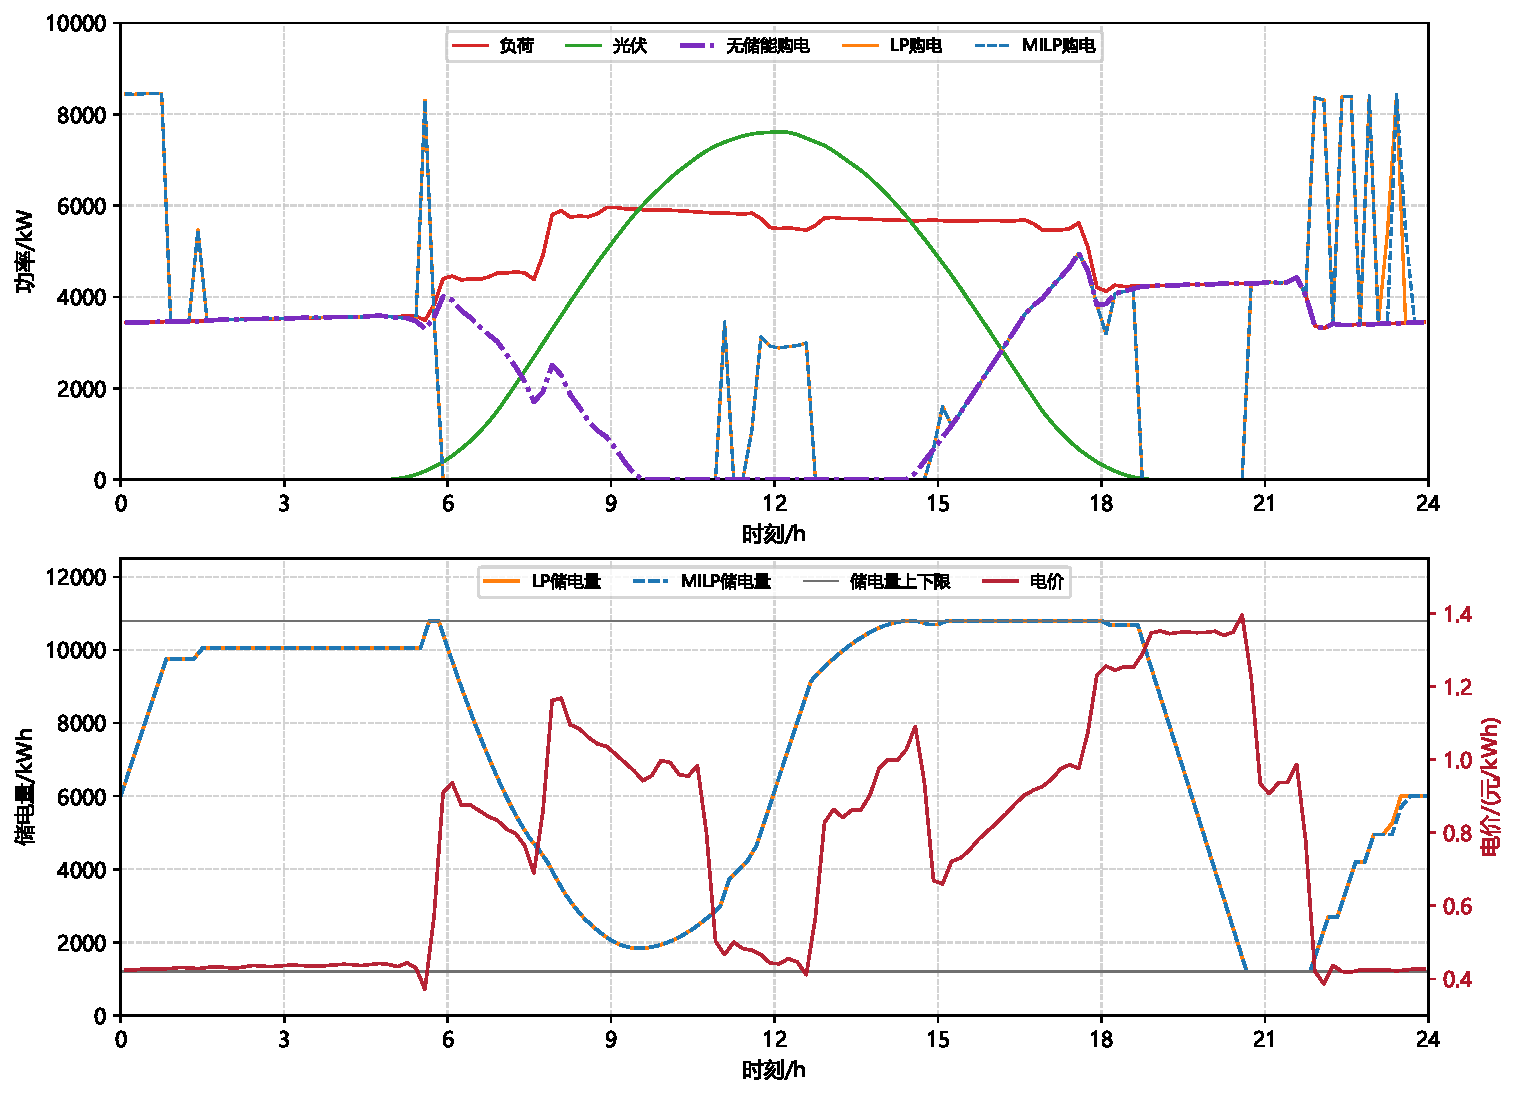
\includegraphics[width=0.72\textwidth]{../figures/问题一/问题一_三种方案调度结果对比.pdf}
  \caption{问题一三种方案的调度结果对比}
  \label{fig:q1_compare}
\end{figure}

由表 4 可见，配置储能设备后全天购电费用下降 26.90\%，弃光量由 6247.96 kWh 降为 0，全天购电量也略有减少。储能设备一方面通过峰谷电价套利降低了高价时段的购电量，另一方面吸收了午间富余的光伏电量，两方面收益共同覆盖了充放电过程中的效率损失。

连续线性规划与混合整数规划的最优费用与全天汇总量完全一致，说明连续松弛在本数据下已经给出了满足充放电互斥条件的最优方案，显式加入 0--1 变量并未改变最优值，只提供了结构上的互斥保证。两种方案在 23:10--23:20 与 23:30--23:40 两个时段的轨迹略有差异，但两时段电价相同，充电量可在其间等价移动，属于多重最优解导致的等价调度方案。

\FloatBarrier
\section{问题二的模型建立与求解}

\subsection{总体思路}

问题二在每天 0:00 一次性确定当天 144 个时段的计划购电量与储能策略，负荷与光伏尚未揭晓时的缺口按 5 倍电价紧急购电。本文按``周期加权预测—整日联合残差场景—季节终端软区间混合整数规划—实际回放结算''的链条求解：所有预测和场景均只用历史信息，日末储电量传递至次日。正式期为 2025 年 2 月 1 日至 12 月 31 日，1 月仅用于构造历史残差和风险窗口。

\subsection{信息边界}

设 $d$ 为计划日期，在 $d$ 日 0:00 可用的信息集为

\begin{equation}
  \mathcal{I}_d = \{\, L_r(t),\ P_r(t) \mid r < d,\ t = 1,2,\dots,144 \,\},
  \label{eq:infoset}
\end{equation}

式中：$L_r(t)$ 与 $P_r(t)$ 分别为历史日期 $r$、时段 $t$ 的实际负荷电量与实际光伏电量；$\mathcal{I}_d$ 只包含 $d$ 日之前已经发生的数据。所有预测、残差归档、场景抽样与终端基准的风险微调均严格限制在 $\mathcal{I}_d$ 之内，当天实际值仅用于计划制定之后的紧急购电结算，以避免未来信息泄漏人为降低回测费用。

\subsection{24 小时周期加权平均预测模型}

附件 2 的实测数据表明，小区负荷具有明显的星期周期，而光伏发电由日内太阳辐照周期主导。据此，本文对负荷采用周周期加权平均、对光伏采用日周期加权平均，并用指数衰减系数对不同历史周期赋权\cite{ref4}。

\subsubsection{负荷预测}

对计划日 $d$ 的时段 $t$，取最近至多 4 个同星期历史时段的指数加权平均：

\begin{equation}
  \widehat{L}_d(t) = \frac{\displaystyle\sum_{k=1}^{K^L_d} \rho^{\,k-1} L_{d-7k}(t)}{\displaystyle\sum_{k=1}^{K^L_d} \rho^{\,k-1}},
  \qquad
  K^L_d = \min\left\{4,\ \left\lfloor \frac{d-1}{7} \right\rfloor \right\}.
  \label{eq:loadpred}
\end{equation}

式中：$\widehat{L}_d(t)$ 为计划日 $d$、时段 $t$ 的负荷电量预测值（kWh）；$L_{d-7k}(t)$ 为前第 $k$ 个同星期同期的实际负荷电量；$\rho$ 为衰减系数，取 0.8；$K^L_d$ 为可用历史周期数。当历史数据达到四周时，式~\eqref{eq:loadpred} 简化为 $L_{d-7},L_{d-14},L_{d-21},L_{d-28}$ 的加权平均，权重依次为 $1,0.8,0.8^2,0.8^3$。每个时段独立计算，不施加相邻时段平滑、样条或误差修正等额外处理。

\subsubsection{光伏预测}

对计划日 $d$ 的时段 $t$，取最近至多 7 个历史日同一时段的指数加权平均：

\begin{equation}
  \widehat{P}_d(t) = \frac{\displaystyle\sum_{k=1}^{K^P_d} \rho^{\,k-1} P_{d-k}(t)}{\displaystyle\sum_{k=1}^{K^P_d} \rho^{\,k-1}},
  \qquad
  K^P_d = \min\{7,\ d-1\}.
  \label{eq:pvpred}
\end{equation}

式中：$\widehat{P}_d(t)$ 为光伏电量预测值（kWh）；$P_{d-k}(t)$ 为前第 $k$ 日的实际光伏电量；$K^P_d$ 为可用历史天数，至多 7 天。考虑光伏出力的非负性，对预测值作非负保护 $\widehat{P}_d(t) \leftarrow \max\{\widehat{P}_d(t), 0\}$。

\subsection{24 小时联合残差场景生成}

点预测无法反映预测误差的分布特征。为在优化中刻画不确定性，本文按整日联合抽样构造场景\cite{ref3}。对历史预测日 $r$，待实际值全部揭晓后归档当日 0:00 实际发出的样本外残差：

\begin{equation}
  e^L_r(t) = L_r(t) - \widehat{L}_r(t), \qquad e^P_r(t) = P_r(t) - \widehat{P}_r(t),
  \label{eq:residual}
\end{equation}

式中：$e^L_r(t)$ 与 $e^P_r(t)$ 分别为历史日期 $r$、时段 $t$ 的负荷与光伏预测残差（kWh）。二者必须来自同一预测日，并以完整的 144 时段日块联合保存，以保留负荷误差与光伏误差之间以及日内各时段误差之间的相关性。

在 $d$ 日 0:00，只使用 $r<d$ 且已完成结算的残差块，历史日期 $r$ 的抽样权重为

\begin{equation}
  \omega_{d,r} = 0.98^{\,d-r} \left[\, 1 + \mathbf{1}\{\operatorname{weekday}(d) = \operatorname{weekday}(r)\} \,\right],
  \label{eq:weight}
\end{equation}

式中：$\omega_{d,r}$ 为历史日期 $r$ 的抽样权重；$0.98^{\,d-r}$ 使时间距离越远的历史日权重越小；$\mathbf{1}\{\cdot\}$ 为指示函数，当历史日与计划日同属一个星期日类型时取 1。将权重归一化后有放回抽取 $S=100$ 个完整日残差块，各场景取等概率 $\pi_s = 1/S$。场景电量为

\begin{equation}
  L_{d,s}(t) = \max\{\widehat{L}_d(t) + e^L_s(t),\ 0\},
  \qquad
  P_{d,s}(t) = \min\left\{ P^{\max}_{d-1},\ \max\{\widehat{P}_d(t) + e^P_s(t),\ 0\} \right\},
  \label{eq:scenario}
\end{equation}

式中：$L_{d,s}(t)$ 与 $P_{d,s}(t)$ 分别为计划日 $d$、场景 $s$、时段 $t$ 的负荷电量与光伏电量（kWh）；$P^{\max}_{d-1}$ 为截至 $d-1$ 日已观测到的最大单时段光伏电量。每日随机种子取日期的八位整数形式，保证同一环境下结果完全可复现。本文取场景数 $S=100$；进一步增大场景数可使期望费用更稳定，但混合整数规划的规模与求解时间随之成倍增长，故不再增加。

\subsection{季节余弦终端软区间的场景混合整数线性规划模型}

\subsubsection{决策变量与场景电量平衡}

计划购电量 $G_d(t)$、充电量 $C_d(t)$、放电量 $D_d(t)$、时段末储电量 $B_d(t)$ 与充放电状态 $z_d(t)$ 在当天 0:00 确定，并在全部场景间共享；紧急购电量 $H_{d,s}(t)$ 与富余电量 $W_{d,s}(t)$ 随场景变化。对任意场景 $s$ 与时段 $t$，供电与用电必须平衡：

\begin{equation}
  G_d(t) + H_{d,s}(t) + P_{d,s}(t) + D_d(t) = L_{d,s}(t) + C_d(t) + W_{d,s}(t),
  \label{eq:q2_balance}
\end{equation}

式中：$H_{d,s}(t)$ 为场景 $s$ 下的紧急购电量（kWh）；$W_{d,s}(t)$ 为场景 $s$ 下无法消纳的富余电量（kWh），其目标系数为 0，不能对外出售，也不能冲减已经承诺的计划购电费用。

\subsubsection{储能约束}

储能状态递推与运行边界为

\begin{equation}
  B_d(t) = B_d(t-1) + \eta_C\,C_d(t) - \frac{D_d(t)}{\eta_D},
  \qquad
  1200 \le B_d(t) \le 10800,
  \label{eq:q2_soc}
\end{equation}

式中：$B_d(0)$ 为当天 0:00 的实际储电量（kWh），由前一天日末储电量传递而来。充放电互斥由 0--1 变量显式保证：

\begin{equation}
  0 \le C_d(t) \le E_{\max}\,z_d(t), \qquad
  0 \le D_d(t) \le E_{\max}\,[1 - z_d(t)], \qquad
  z_d(t) \in \{0,1\},
  \label{eq:q2_mutex}
\end{equation}

式中：$z_d(t)$ 为充放电状态变量，$z_d(t)=1$ 允许充电、$z_d(t)=0$ 允许放电。

\subsubsection{日末储电量的季节余弦基准与因果风险微调}

24 小时的有限优化时域会使模型倾向把日末储电量放空，而放空的储电量在次日需要以更高代价重新购入。固定的日末备用目标无法反映负载与光伏的年周期变化，因此本文改用随季节变化、并由当日场景风险因果微调的终端软区间；固定目标或不设终端约束都会让日末储电量被压在某一常数或运行下限上，全年费用明显更高，三者对照见后文。

（1）季节余弦基准。计及负荷与光伏的年周期，令日末储电量的季节基准为

\begin{equation}
  B_d^{\mathrm{season}} = 7000 + 800\cos\!\left[\frac{2\pi\left(\operatorname{doy}(d) - 15\right)}{365}\right],
  \label{eq:q2_season}
\end{equation}

式中：$\operatorname{doy}(d)\in[1,365]$ 为计划日 $d$ 在一年中的序号；基准在 1 月中旬取最大值 7800 kWh，在 7 月中旬取最小值 6200 kWh，与冬季负荷高、光伏低的运行特征一致。

（2）因果风险微调。当日 0:00 的 100 个联合场景已经刻画了当天的净负荷风险，定义风险分数

\begin{equation}
  \xi_d = Q_{0.80}\!\left(\sum_{t=1}^{144}\left(L_{d,s}(t)-P_{d,s}(t)\right)\right)
  - \operatorname{mean}_s\!\left(\sum_{t=1}^{144}\left(L_{d,s}(t)-P_{d,s}(t)\right)\right),
  \label{eq:q2_riskscore}
\end{equation}

式中：$\xi_d$ 为当日风险分数（kWh），取各场景净负荷总量的 80\% 分位数与其均值之差，用于度量场景分布的右尾厚度。记此前至多 56 日的风险分数所成序列为 $\{\xi_{d'}\mid d-56\le d'<d\}$，并取其滚动中位数与稳健尺度

\begin{equation}
  \operatorname{med}_{56} = \operatorname{median}\{\xi_{d'}\}, \qquad
  \sigma_{56} = 1.4826\,\operatorname{MAD}\{\xi_{d'}\},
  \label{eq:q2_medmad}
\end{equation}

式中：$\operatorname{median}$ 与 $\operatorname{MAD}$ 分别为中位数与中位数绝对偏差；1.4826 为使其无偏估计正态标准差的一致性系数；为保证数值稳定，$\sigma_{56}$ 的下限取 100 kWh。在式~\eqref{eq:q2_medmad} 的基础上，当日调整量取

\begin{equation}
  \delta_d = \operatorname{clip}\!\left(\frac{200\,(\xi_d - \operatorname{med}_{56})}{\sigma_{56}},\ -600,\ +600\right),
  \label{eq:q2_riskadj}
\end{equation}

式中：200 kWh 为每单位风险尺度对应的调整量；$\pm600$ kWh 为截断界限。风险分数高于历史中位数时上调终端基准，低于中位数时下调，全部依据此前已发生的信息，不含未来信息。

（3）终端软区间与偏离量。最终参考值取

\begin{equation}
  B_d^{\mathrm{ref}} = \operatorname{clip}\!\left(B_d^{\mathrm{season}} + \delta_d,\ 5200,\ 8600\right),
  \label{eq:q2_ref}
\end{equation}

式中：$[5200,8600]$ 为参考值的截断区间（kWh）。终端软区间为 $[B_d^{\mathrm{ref}}-1000,\ B_d^{\mathrm{ref}}+1000]$。引入下沿不足量 $R_d$ 与上沿超出量 $X_d$：

\begin{equation}
  R_d \ge B_d^{\mathrm{ref}} - 1000 - B_d(144), \qquad R_d \ge 0,
  \label{eq:q2_lower}
\end{equation}

\begin{equation}
  X_d \ge B_d(144) - \left(B_d^{\mathrm{ref}} + 1000\right), \qquad X_d \ge 0,
  \label{eq:q2_upper}
\end{equation}

式中：$B_d(144)$ 为当天 24:00 的储电量（kWh）；$R_d$ 与 $X_d$ 分别为日末储电量低于下沿与高于上沿的部分（kWh）。

（4）目标函数。单日模型的目标函数为

\begin{equation}
  \min\ Z_2 = \underbrace{\sum_{t=1}^{144} \lambda(t) G_d(t)}_{\text{计划购电费}}
  + \underbrace{\sum_{s=1}^{S} \pi_s \sum_{t=1}^{144} 5\lambda(t) H_{d,s}(t)}_{\text{期望紧急购电费}}
  + \underbrace{\kappa\,(R_d + X_d)}_{\text{终端偏离惩罚}}.
  \label{eq:q2_obj}
\end{equation}

式中：第一项为按计划购电量结算的购电费（元）；第二项为各场景紧急购电费的期望，紧急购电电价为对应时段正常电价的 5 倍；第三项为终端储电量偏离软区间的机会成本，惩罚系数取

\begin{equation}
  \kappa = \eta_D\, Q_{0.90}(\lambda) = 0.9 \times 1.2500 = 1.1250\ \text{元/kWh},
  \label{eq:kappa}
\end{equation}

式中：$\eta_D$ 为放电效率；$Q_{0.90}(\lambda)$ 为固定日内电价的 90\% 分位数（元/kWh）。由于固定日内电价在每天 0:00 已知，$\kappa$ 的计算不使用未来的实际负荷、实际光伏或紧急购电信息；终端偏离惩罚只用于优化决策，不计入实际支付费用。

\subsection{跨日储电量传递}

正式期自 2025 年 2 月 1 日 0:00 开始，初始储电量取 6000 kWh；此后不设置每日首末相等或年末回到固定值的硬性约束，日末储电量按 $B_d(0) = B_{d-1}(144)$ 连续传递至次日。2025 年 1 月不作为优化区间，只用于积累样本外残差场景库以及为风险微调提供历史窗口。

\subsection{实际执行与费用结算}

当天实际负荷与实际光伏揭晓后，计划量 $G_d(t),C_d(t),D_d(t)$ 保持不变，实际紧急购电量按资源缺口回放计算：

\begin{equation}
  H_d^{\mathrm{act}}(t) = \max\{\, L_d(t) + C_d(t) - G_d(t) - P_d(t) - D_d(t),\ 0 \,\},
  \label{eq:q2_actual}
\end{equation}

式中：$H_d^{\mathrm{act}}(t)$ 为实际紧急购电量（kWh）。当天实际费用为

\begin{equation}
  F_d^{\mathrm{act}} = \sum_{t=1}^{144} \lambda(t) G_d(t) + \sum_{t=1}^{144} 5\lambda(t) H_d^{\mathrm{act}}(t),
  \label{eq:q2_cost}
\end{equation}

式中：第一项为正常购电费，始终按 0:00 确定的计划量结算；第二项为实际紧急购电费。实际富余电量不予退款，场景期望量也不能替代最终的实际紧急购电量。

\subsection{求解结果与分析}

\subsubsection{负荷与光伏的周期性分析}

按 2025 年公历将全年各日划分为星期一至星期日并求平均，得到各类星期的平均负荷与平均光伏曲线，如图~\ref{fig:q2_weekday} 所示。星期五、星期六的负荷曲线明显低于其他日期，星期日与星期一至星期四处于较高平台；光伏的七条平均曲线形态接近，主要由日内太阳辐照周期控制，说明光伏不具有星期差异。

\begin{figure}[H]
  \centering
  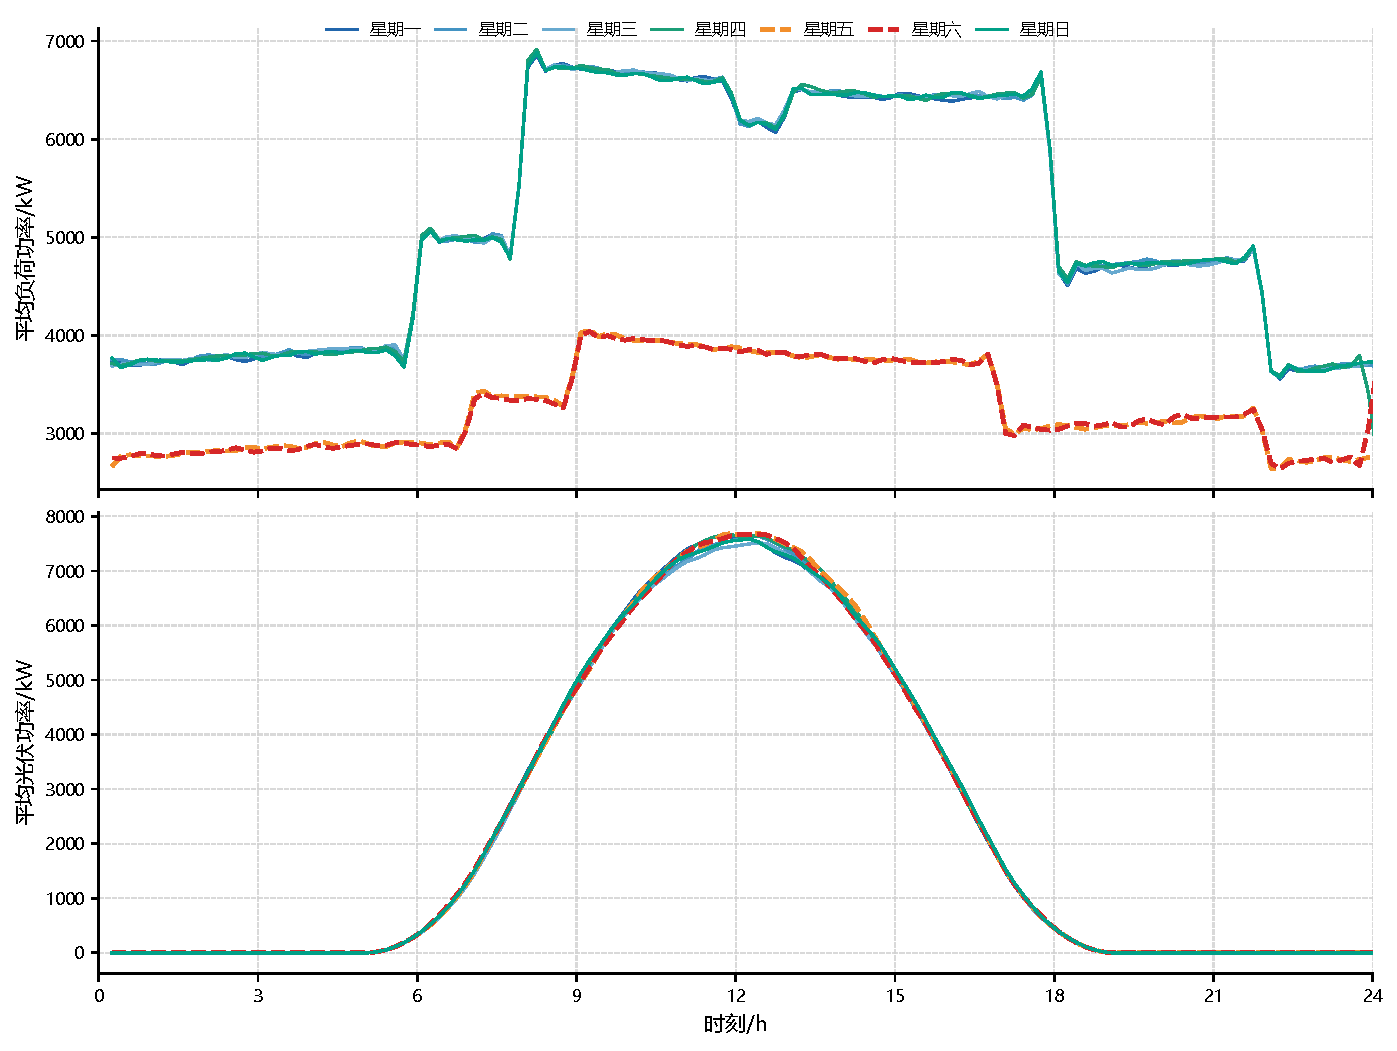
\includegraphics[width=0.72\textwidth]{../figures/问题二/问题二_星期一至星期日平均负荷与光伏曲线.pdf}
  \caption{星期一至星期日的平均负荷与光伏曲线}
  \label{fig:q2_weekday}
\end{figure}

为进一步确认周期结构，对每一天的 144 个时段取日均值，再基于全年 365 个日均值计算日尺度自相关函数，结果如图~\ref{fig:q2_acf} 所示。日均负荷在滞后 1 天、7 天与 14 天的自相关系数分别为 0.3732、0.9710 与 0.9424，后两者显著高于其余滞后，支持采用 7 天负荷周期；日均光伏对应为 0.9562、0.8780 与 0.7684，滞后 1 天即具有很高的相关性，支持采用日周期信息预测光伏。

\begin{figure}[H]
  \centering
  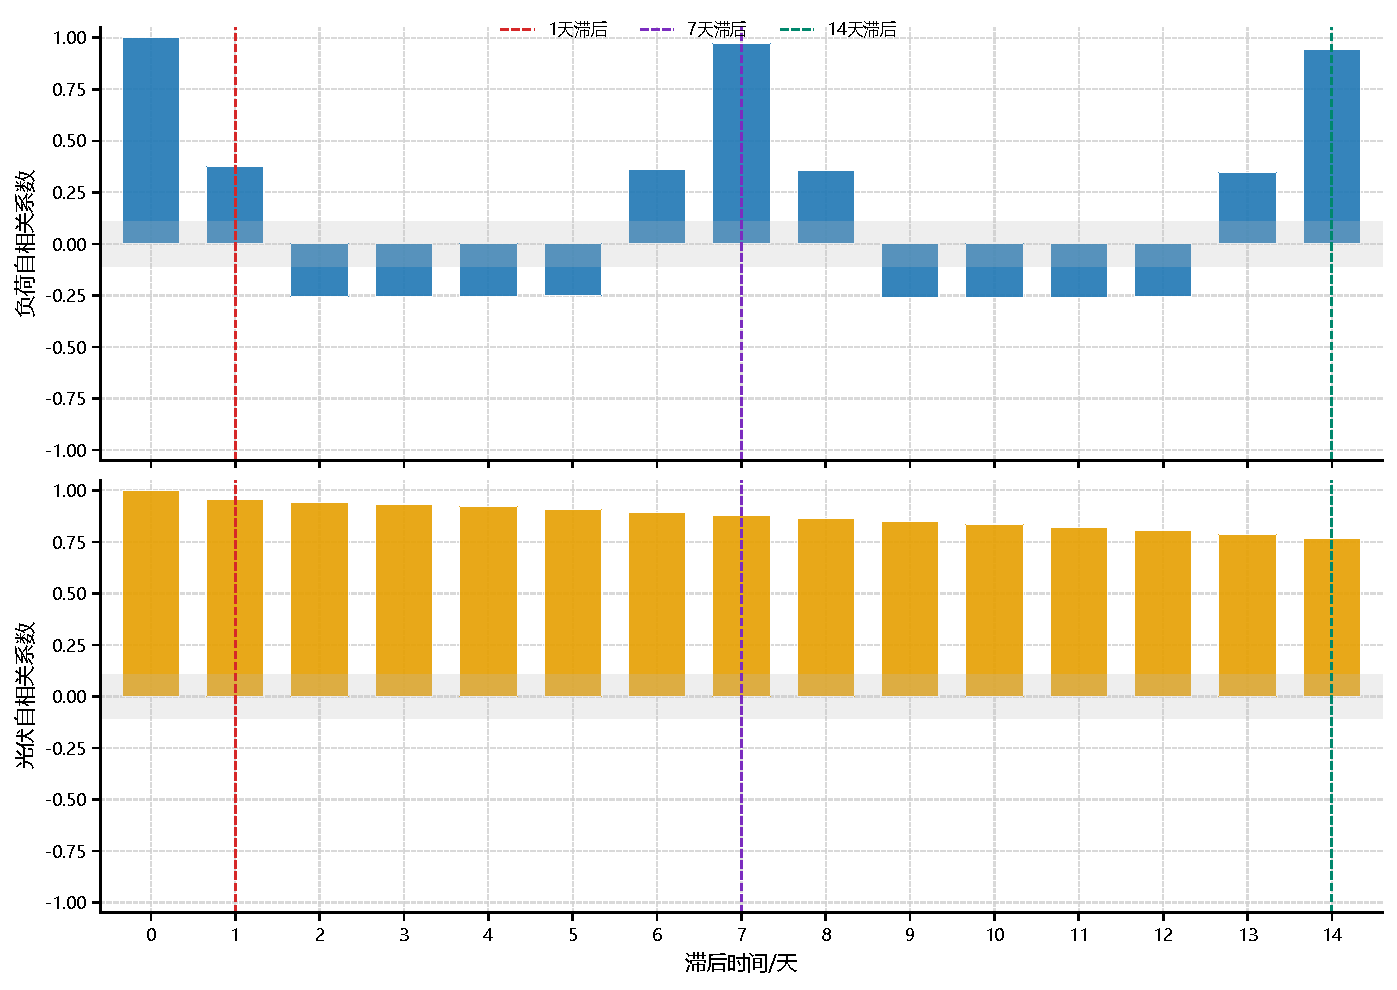
\includegraphics[width=0.72\textwidth]{../figures/问题二/问题二_负荷与光伏ACF.pdf}
  \caption{日均负荷与日均光伏的自相关函数}
  \label{fig:q2_acf}
\end{figure}

\subsubsection{预测精度}

对任一实际序列 $y_i$ 及其预测值 $\widehat y_i$，加权平均绝对百分比误差（WAPE）定义为

\begin{equation}
  \operatorname{WAPE}=\frac{\displaystyle\sum_{i=1}^{n}\left|y_i-\widehat y_i\right|}{\displaystyle\sum_{i=1}^{n}\left|y_i\right|}\times100\%.
  \label{eq:wape}
\end{equation}

式中：$i$ 为时段索引，$n$ 为评价时段数，$y_i$ 与 $\widehat y_i$ 分别为实际值和预测值；本研究中各评价量非负，故分母为评价期实际量总和。

在 2025 年 2 月 1 日至 12 月 31 日共 334 天、48096 个 10 分钟时段上，逐日向前预测的结果为：负荷平均绝对误差 29.902 kWh、均方根误差 41.701 kWh、WAPE 3.89\%；光伏全时段平均绝对误差 24.970 kWh、均方根误差 50.047 kWh、WAPE 6.30\%，非零时段平均绝对误差 44.669 kWh。所有误差均来自严格按时间向前的样本外预测，而非全年拟合后的样本内结果；指定日对比如图~\ref{fig:q2_day} 所示。

\begin{figure}[H]
  \centering
  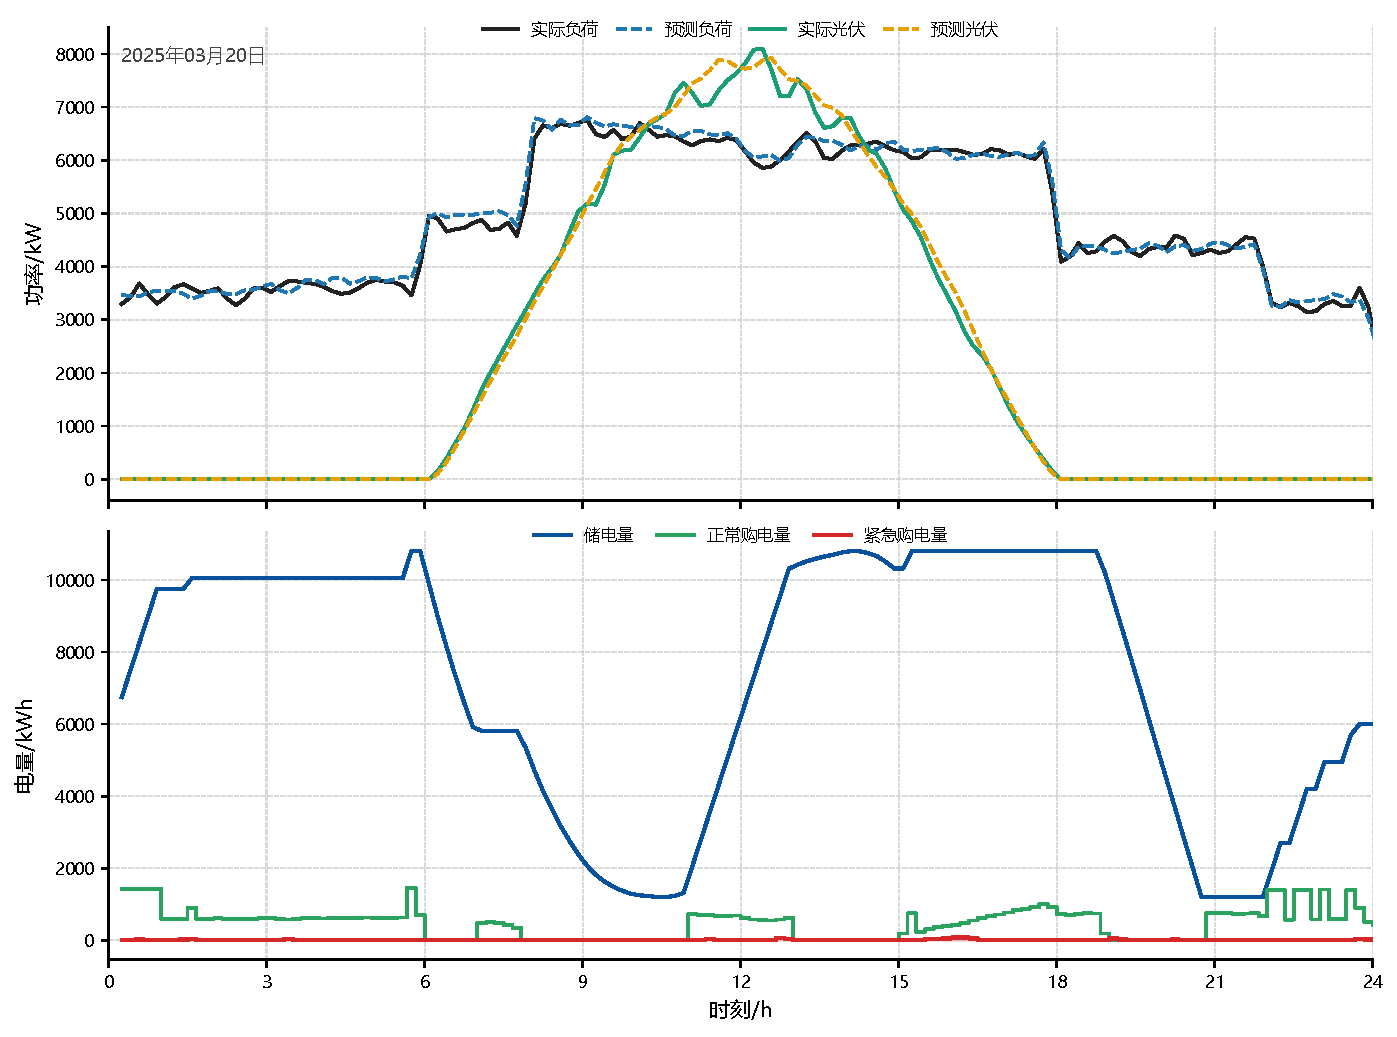
\includegraphics[width=0.72\textwidth]{../figures/问题二/问题二_24小时预测值与实际值.pdf}
  \caption{2025 年 3 月 20 日 24 小时预测值与实际值}
  \label{fig:q2_day}
\end{figure}

图~\ref{fig:q2_month} 给出 3 月日总电量的预测与实际对比，负荷的星期周期与光伏的缓慢季节变化均得到体现。

\begin{figure}[H]
  \centering
  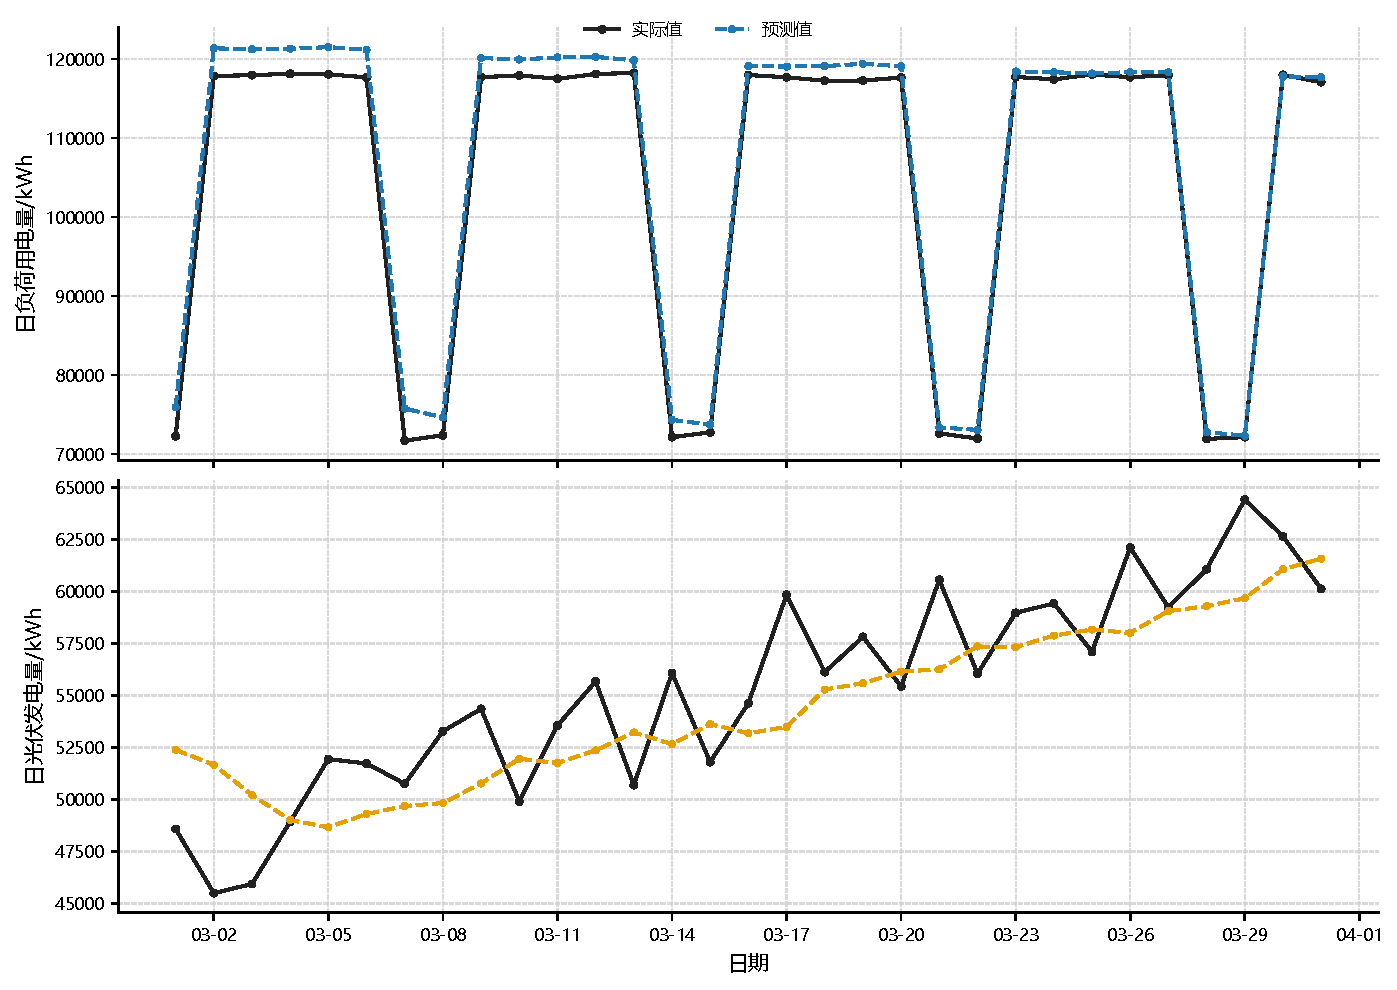
\includegraphics[width=0.72\textwidth]{../figures/问题二/问题二_一个月预测值与实际值.pdf}
  \caption{2025 年 3 月日总电量的预测值与实际值}
  \label{fig:q2_month}
\end{figure}

题目指定日期的完整购电、储能和紧急购电结果见表 6 至表 8。其中，12 月 21 日的计划购电量与购电费用最高，与冬季负荷较高、光伏出力较低的特征一致；储能设备在四个日期均呈现``夜间与午间低价时段充电、早晚高价时段放电''的套利特征。

\subsubsection{全年优化结果}

2025 年 2 月 1 日至 12 月 31 日共 334 天的全年汇总结果如表 5 所示。

{\footnotesize
\threelinetable{表 5\quad 问题二正式期全年汇总结果}{l r l r}{%
  \textbf{指标} & \textbf{结果} & \textbf{指标} & \textbf{结果}%
}{%
  正式天数 & 334 & 紧急购电费/元 & 1170588.48 \\
  计划购电量/kWh & 22069571.55 & 实际总费用/元 & 14637169.37 \\
  实际紧急购电量/kWh & 314788.59 & 平均日末储电量/kWh & 5993.78 \\
  实际富余电量/kWh & 3106105.93 & 日末储电量标准差/kWh & 541.93 \\
  正常购电费/元 & 13466580.90 & 12 月 31 日末储电量/kWh & 6626.15 \\
}
}

全年实际紧急购电量为 314788.59 kWh，约占计划购电量的 1.43\%；紧急购电费为 1170588.48 元，约占实际总费用的 8.00\%。平均日末储电量为 5993.78 kWh，标准差 541.93 kWh，说明日末储电量在季节基准与风险微调的共同作用下围绕软区间下沿小幅波动，而非固定在某一常数。全年逐日的正常购电量、紧急购电量与日末储电量如图~\ref{fig:q2_year} 所示。

\begin{figure}[H]
  \centering
  
\includegraphics[width=0.72\textwidth]{../figures/问题二/问题二_全年正常购电紧急购电与储电量.pdf}
  \caption{全年正常购电量、紧急购电量与日末储电量}
  \label{fig:q2_year}
\end{figure}

\subsubsection{指定日期的完整结果}

指定日期的购电、储能与紧急购电结果分别见表 6 至表 8。

{\scriptsize
\threelinetable{表 6\quad 问题二指定日期的购电结果}{l r r r r}{%
  \textbf{时间段} & \textbf{3 月 20 日} & \textbf{6 月 21 日} & \textbf{9 月 23 日} & \textbf{12 月 21 日}%
}{%
  10:00--10:10 & 0.00 & 0.00 & 0.00 & 0.00 \\
12:00--12:10 & 577.07 & 0.00 & 517.78 & 978.76 \\
14:00--14:10 & 0.00 & 0.00 & 0.00 & 0.00 \\
16:00--16:10 & 483.38 & 200.02 & 559.60 & 859.59 \\
18:00--18:10 & 700.06 & 0.00 & 825.99 & 727.46 \\
20:00--20:10 & 0.00 & 0.00 & 23.26 & 0.00 \\
全天购电量/kWh & 69205.65 & 37039.50 & 73127.51 & 97759.82 \\
全天购电费/元 & 45090.68 & 21942.35 & 47574.23 & 65454.20 \\
}

}

{\tiny
\begin{center}
  {\fontsize{10.5pt}{12.6pt}\heiti\bfseries 表 7\quad 问题二指定日期的储能结果}\par
  \vspace{0.25em}
  \resizebox{\textwidth}{!}{%
  \begin{tabular}{l r r r r r r r r}
    \toprule
    & \multicolumn{2}{c}{\textbf{3 月 20 日}} & \multicolumn{2}{c}{\textbf{6 月 21 日}} & \multicolumn{2}{c}{\textbf{9 月 23 日}} & \multicolumn{2}{c}{\textbf{12 月 21 日}} \\
    \cmidrule(lr){2-3}\cmidrule(lr){4-5}\cmidrule(lr){6-7}\cmidrule(lr){8-9}
    \textbf{时间段} & \textbf{充电量/kWh} & \textbf{放电量/kWh} & \textbf{充电量/kWh} & \textbf{放电量/kWh} & \textbf{充电量/kWh} & \textbf{放电量/kWh} & \textbf{充电量/kWh} & \textbf{放电量/kWh} \\
    \midrule
    0:00-4:00 & 3994.16 & 0.00 & 0.00 & 0.00 & 4701.99 & 0.00 & 3748.89 & 0.00 \\
4:00-8:00 & 833.33 & 5476.96 & 40.51 & 3473.19 & 833.33 & 5589.10 & 1666.67 & 1508.33 \\
8:00-12:00 & 5959.76 & 3163.04 & 6212.03 & 0.00 & 6188.17 & 3050.90 & 5833.33 & 7806.67 \\
12:00-16:00 & 5240.40 & 432.13 & 3794.87 & 0.00 & 4883.90 & 328.38 & 8177.36 & 2708.67 \\
16:00-20:00 & 0.00 & 5683.04 & 0.00 & 5971.81 & 0.00 & 5833.33 & 0.00 & 5620.93 \\
20:00-24:00 & 5806.94 & 2956.96 & 4697.87 & 2668.19 & 4980.19 & 2806.67 & 6478.83 & 3019.07 \\
0:00 储电量/kWh & \multicolumn{2}{c}{6455.25} & \multicolumn{2}{c}{5616.43} & \multicolumn{2}{c}{5818.21} & \multicolumn{2}{c}{6676.00} \\
24:00 储电量/kWh & \multicolumn{2}{c}{6426.24} & \multicolumn{2}{c}{5428.08} & \multicolumn{2}{c}{5682.17} & \multicolumn{2}{c}{7030.95} \\
    \bottomrule
  \end{tabular}%
  }
\end{center}
}

{\scriptsize
\threelinetable{表 8\quad 问题二指定日期的紧急购电结果}{l r l r l r l r}{%
  \textbf{3 月 20 日 时段} & \textbf{购电量/kWh} & \textbf{6 月 21 日 时段} & \textbf{购电量/kWh} & \textbf{9 月 23 日 时段} & \textbf{购电量/kWh} & \textbf{12 月 21 日 时段} & \textbf{购电量/kWh}%
}{%
  0:30-0:40 & 23.88 & 0:30-0:40 & 37.44 & 5:10-5:20 & 11.27 & 1:10-1:30 & 18.00 \\
1:10-1:50 & 57.91 & 1:30-1:40 & 40.00 & 5:50-6:00 & 1.20 & 1:40-2:00 & 18.50 \\
2:40-2:50 & 5.46 & 2:00-2:20 & 16.74 & 6:20-6:30 & 0.94 & 2:20-2:30 & 12.93 \\
3:10-3:40 & 73.60 & 3:00-3:40 & 62.95 & 7:00-7:10 & 5.93 & 3:10-3:30 & 54.51 \\
5:10-5:20 & 6.05 & 6:10-6:20 & 15.64 & 9:50-10:20 & 49.27 & 3:40-4:10 & 106.83 \\
10:00-10:10 & 4.85 & 19:10-19:20 & 21.22 & 11:00-11:10 & 42.26 & 4:20-4:30 & 0.23 \\
11:10-11:30 & 42.83 & 20:30-20:40 & 6.87 & 14:40-15:30 & 214.72 & 5:50-6:40 & 87.72 \\
12:40-13:00 & 90.14 &  &  & 16:00-16:20 & 58.72 & 10:30-11:50 & 451.32 \\
15:20-17:20 & 382.19 &  &  & 16:40-17:00 & 9.59 & 13:00-13:20 & 20.00 \\
18:20-18:30 & 2.55 &  &  & 20:30-20:40 & 10.11 & 17:30-17:40 & 7.98 \\
18:50-19:20 & 88.21 &  &  & 21:00-21:10 & 40.94 & 18:30-18:40 & 2.68 \\
20:00-20:30 & 24.35 &  &  & 22:30-22:40 & 6.00 & 18:50-19:10 & 4.07 \\
21:30-21:50 & 19.43 &  &  &  &  & 19:50-20:10 & 52.37 \\
23:40-0:00+1 & 55.73 &  &  &  &  & 23:00-23:10 & 9.65 \\
 &  &  &  &  &  & 23:40-23:50 & 0.61 \\
}
}


\subsubsection{终端储电量机制的对照分析}

在同一预测、随机种子和联合残差场景下，对四种终端处理方式进行对照。无终端约束、固定 6000 kWh 基准、季节余弦基准及季节基准叠加因果微调的全年费用依次为 14651641.38、14640006.24、14637301.67 和 14637169.37 元；对应的逐步节省额为 11635.14、2704.57 和 132.30 元。季节基准的贡献明显大于风险微调，说明终端机制主要避免跨日储能透支。

风险微调在正式期上调 189 天、下调 145 天，16 天触及 $+600$ kWh 截断上限，调整均值为 67.15 kWh。334 天的日末储电量均贴近当日软区间下沿，范围为 5105.04$\sim$7196.85 kWh，表明其作用是因果移动季节性最低备用曲线。四种方案的费用与储电量对比如图~\ref{fig:q2_reserve} 所示。

\begin{figure}[H]
  \centering
  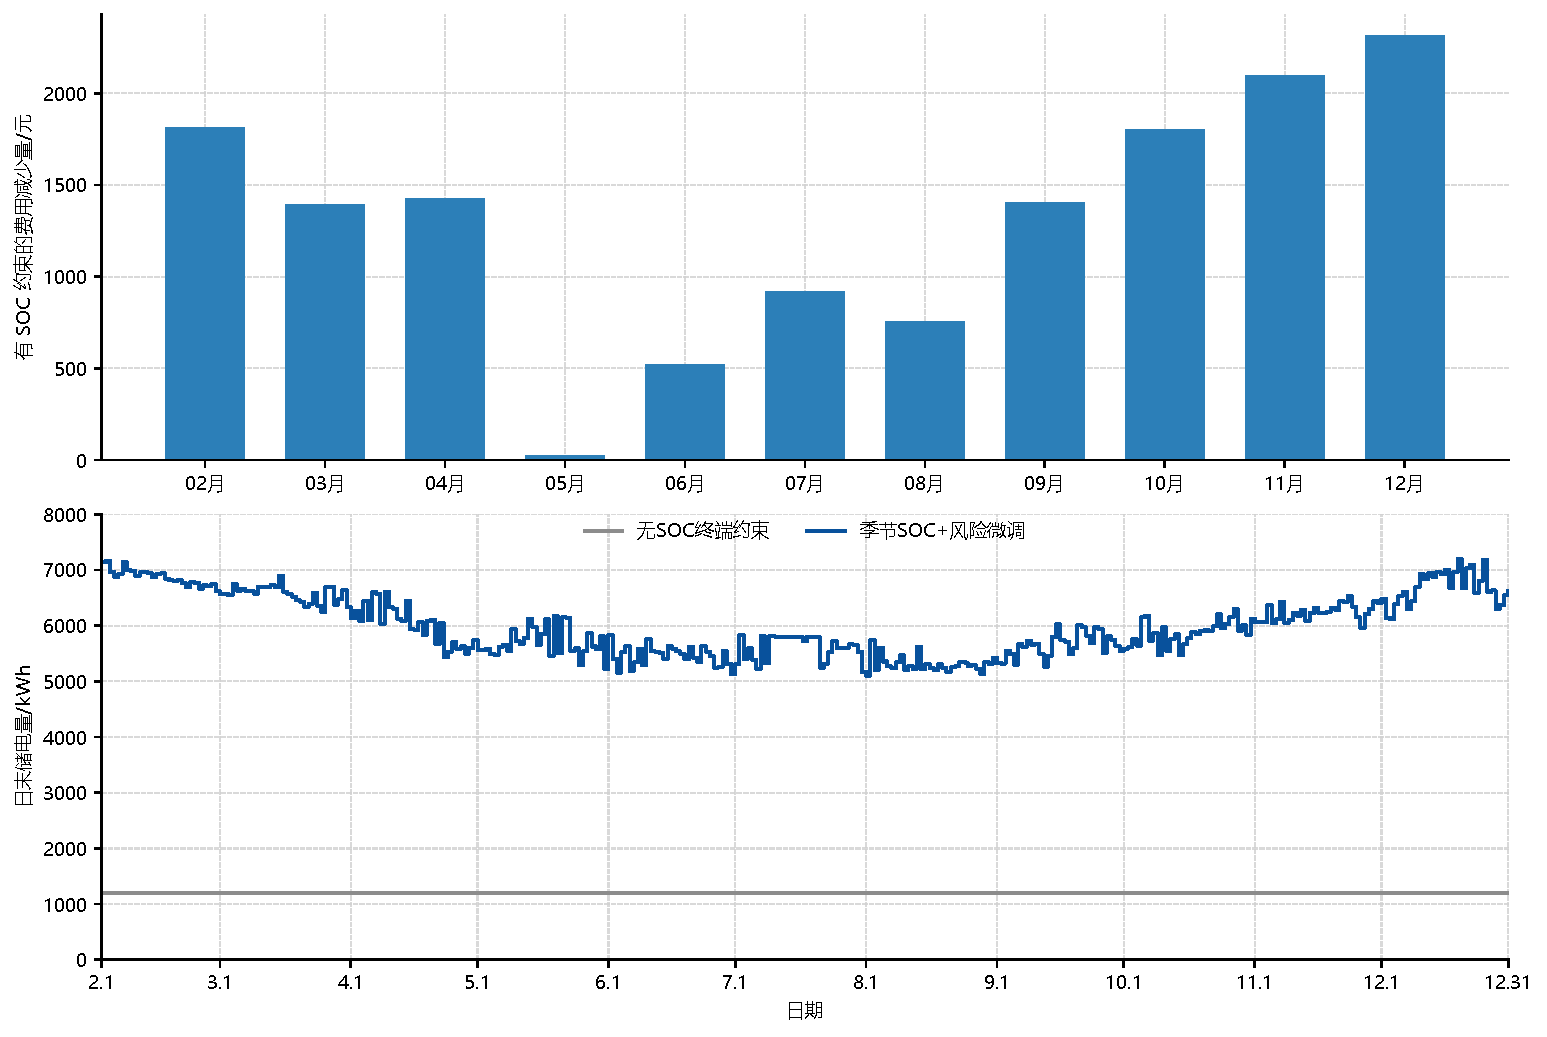
\includegraphics[width=0.72\textwidth]{../figures/问题二/问题二_日备不足惩罚前后费用与储能对比.pdf}
  \caption{有、无终端储电量约束方案的费用与日末储电量对比}
  \label{fig:q2_reserve}
\end{figure}

\FloatBarrier
\section{问题三的模型建立与求解}

\subsection{光伏预报数据的插值与时间匹配}

附件 3 提供 2025 年全年每天 0:00、6:00、12:00、18:00 四个发布时点、每次发布未来 24 个整点的光伏发电功率预报，共 $365\times4\times24$ 条记录。设发布时点为 $\tau\in\{0,6,12,18\}$，字段``预报 $k$ 小时''对应发布时间之后第 $k$ 个整点。以发布时刻已经观测到的实际光伏功率为左端点，与未来 24 个整点预报一起构成插值节点，分段线性插值到 10 分钟网格后乘以 $\Delta t = 1/6$ h，得到 10 分钟尺度的光伏电量预测：

\begin{equation}
  \widehat{P}^{(\tau)}_d(t) = \frac{1}{6}\,\mathrm{interp}\left(\tau,\, t\right),
  \label{eq:q3_pv}
\end{equation}

式中：$\tau$ 为预报的发布时点；$\widehat{P}^{(\tau)}_d(t)$ 为计划日 $d$、时段 $t$ 由时点 $\tau$ 的预报生成的光伏电量预测（kWh）；$\mathrm{interp}(\cdot)$ 为分段线性插值的功率结果（kW）。

以附件 2 的时刻列作为执行边界：6:00 的更新只能修改结束时刻晚于 6:00 的时段，12:00 与 18:00 同理。日内不更新负荷预测，因为附件 3 只提供光伏预报，负荷仍沿用问题二的周周期加权平均预测。

\subsection{发布时间匹配的联合残差场景}

问题三的联合残差场景需在每个发布时点分别构造。对历史日 $r$ 与发布时点 $\tau$，归档当日在该时点实际发出的样本外残差：

\begin{equation}
  e^L_r(t) = L_r(t) - \widehat{L}_r(t),
  \qquad
  e^{P,\tau}_r(t) = P_r(t) - \widehat{P}^{(\tau)}_r(t),
  \label{eq:q3_residual}
\end{equation}

式中：$e^L_r(t)$ 为负荷预测残差（kWh）；$e^{P,\tau}_r(t)$ 为由时点 $\tau$ 预报生成的光伏预测残差（kWh）。

在计划日 $d$ 的发布时点 $\tau$，只允许使用 $r<d$ 且实际值已全部揭晓的完整同日残差块，历史日权重与问题二一致：

\begin{equation}
  \omega_{d,r} = 0.98^{\,d-r}\left[\,1 + \mathbf{1}\{\operatorname{weekday}(d)=\operatorname{weekday}(r)\}\,\right].
  \label{eq:q3_weight}
\end{equation}

将权重归一化后有放回抽取 100 次，取经验频数为场景概率；完全相同的重复历史日场景在实现中合并并按出现频数赋权，这与保留 100 份重复变量严格等价，但显著降低了混合整数规划的规模。场景电量为

\begin{equation}
  L^{(\tau)}_{d,s}(t) = \max\{\widehat{L}_d(t) + e^L_s(t),\ 0\},
  \qquad
  P^{(\tau)}_{d,s}(t) = \max\{\widehat{P}^{(\tau)}_d(t) + e^{P,\tau}_s(t),\ 0\},
  \label{eq:q3_scenario}
\end{equation}

式中：$L^{(\tau)}_{d,s}(t)$ 与 $P^{(\tau)}_{d,s}(t)$ 分别为时点 $\tau$ 下、场景 $s$、时段 $t$ 的负荷电量与光伏电量（kWh）；光伏场景上界只使用当前发布时点以前已经观测到的最大光伏电量。

\subsection{0:00 原计划模型}

0:00 原计划模型与问题二完全一致：场景电量平衡同式~\eqref{eq:q2_balance}，储能状态递推与容量边界同式~\eqref{eq:q2_soc}，充放电互斥同式~\eqref{eq:q2_mutex}，终端软区间同式~\eqref{eq:q2_lower} 与式~\eqref{eq:q2_upper}（其中季节基准 $B_d^{\mathrm{season}}$ 与风险调整量 $\delta_d$ 由式~\eqref{eq:q2_season}、式~\eqref{eq:q2_riskadj} 给出）。区别只有一处：光伏场景改由附件 3 的预报生成，即式~\eqref{eq:q2_balance} 中的 $P_{d,s}(t)$ 取 $P^{(0)}_{d,s}(t)$。0:00 的目标函数为

\begin{equation}
  \min\left\{
    \sum_t \lambda(t) G_d(t)
    + \sum_s \pi_s \sum_t 5\lambda(t) H_{d,s}(t)
    + 1.1250\,\bigl(R_d + X_d\bigr)
  \right\},
  \label{eq:q3_obj0}
\end{equation}

式中：三项依次为计划购电费、期望紧急购电费与终端偏离惩罚（元），其含义与式~\eqref{eq:q2_obj} 一致。

\subsection{日内滚动调整模型}

对发布时点 $\tau \in \{6,12,18\}$，设重新优化后的购电量为 $A^{(\tau)}(t)$，相对 0:00 原计划的调整量为

\begin{equation}
  A^{(\tau)}(t) - G(t) = U^{(\tau)}(t) - V^{(\tau)}(t),
  \qquad
  A^{(\tau)}(t),\,U^{(\tau)}(t),\,V^{(\tau)}(t) \ge 0,
  \label{eq:q3_adjust}
\end{equation}

式中：$A^{(\tau)}(t)$ 为调整后购电量（kWh）；$U^{(\tau)}(t)$ 与 $V^{(\tau)}(t)$ 分别为相对原计划的上调量与下调量（kWh），二者是与终端偏离量 $R_d$、$X_d$ 无关的另一组变量。采用净结算口径：上调部分按 1.5 倍电价计费，下调取消部分按 50\% 电价承担违约费用，即时段结算费为

\begin{equation}
  F_t^{\mathrm{sch}} = \lambda(t)G(t) + 1.5\lambda(t)U^{(\tau)}(t) - 0.5\lambda(t)V^{(\tau)}(t),
  \label{eq:q3_schedule_cost}
\end{equation}

由于同一时段同时上调和下调只会增加费用，最优解中二者不会并存。若把下调理解为``计划量全额付费并另加 50\% 违约费''，下调的边际成本将由 0.5 倍电价升至 1.5 倍电价，滚动调整的幅度会明显减小，日内更新的价值会被低估。

剩余时域 $\mathcal T_\tau$ 上的场景电量平衡为

\begin{equation}
  A^{(\tau)}(t) + H^{(\tau)}_s(t) + P^{(\tau)}_s(t) + D^{(\tau)}(t)
  = L_s(t) + C^{(\tau)}(t) + W^{(\tau)}_s(t),
  \qquad t \in \mathcal T_\tau,
  \label{eq:q3_rolling_balance}
\end{equation}

式中：$\mathcal T_\tau$ 为发布时点 $\tau$ 之后尚未执行的时段集合。储能约束与 0:00 模型相同，但初始储电量改为当前实际已执行的储电量。去掉式~\eqref{eq:q3_schedule_cost} 中不随决策变化的常数项 $\sum_t\lambda(t)G(t)$ 后，滚动优化的目标函数为

\begin{equation}
  \begin{aligned}
    \min\Biggl\{
      &\sum_{t\in\mathcal T_\tau}\left[1.5\lambda(t)U^{(\tau)}(t) - 0.5\lambda(t)V^{(\tau)}(t)\right] \\
      &\quad + \sum_s \pi_s \sum_{t\in\mathcal T_\tau} 5\lambda(t) H_s(t)
      + 1.1250\,\bigl(R_d^{(\tau)} + X_d^{(\tau)}\bigr)\Biggr\}.
  \end{aligned}
  \label{eq:q3_objroll}
\end{equation}

式中：$R_d^{(\tau)}$ 与 $X_d^{(\tau)}$ 为该时点优化得到的终端偏离量（kWh）。富余电量的目标系数为 0，实现中把它从决策变量中消去、以不等式 $H \ge L + C - A - P - D$ 表示场景缺口，求解后由正部恢复富余量，该处理不改变可行域与最优值。

\subsection{滚动执行与实际费用结算}

四种待比较的策略为：仅 0:00；增加 6:00；增加 6:00 与 12:00；使用全部四时点。每次更新都把模型求解到当天 24:00，但只执行到下一个启用时点，已发生的购电量、充放电量与储电量不允许回溯修改。最终拼接得到的购电量、充电量、放电量记为 $A^{\mathrm{exec}},C^{\mathrm{exec}},D^{\mathrm{exec}}$。

当天实际值揭晓后，实际紧急购电量为

\begin{equation}
  H_d^{\mathrm{act}}(t) = \max\{L_d(t) + C^{\mathrm{exec}}_d(t) - A^{\mathrm{exec}}_d(t) - P_d(t) - D^{\mathrm{exec}}_d(t),\ 0\}.
  \label{eq:q3_actual}
\end{equation}

需要说明的是，本文报告的是实际富余电量 $W^{\mathrm{act}}_d(t)$，即无法被负荷、充电与储能共同消纳的电量；按``出现富余时优先削减光伏''的口径，其中不超过同期实际光伏发电量的部分才是弃光，本文不再单独列出这一拆分。实际总费用为

\begin{equation}
  F^{\mathrm{total}} = \sum_{d,t}\left[\lambda G + 1.5\lambda U - 0.5\lambda V + 5\lambda H^{\mathrm{act}}\right],
  \label{eq:q3_total_cost}
\end{equation}

式中：四项依次为计划购电费、上调加价费、下调抵扣（负值）与实际紧急购电费（元）。终端偏离惩罚只用于优化决策，不计入实际支付费用。

\subsection{求解结果与分析}

\subsubsection{官方光伏预报的精度评价}

为避免不同剩余时域造成的偏差，按相同目标 6 小时区段比较各发布时点可用预报的平均绝对误差，结果如图~\ref{fig:q3_pv_err} 所示，每组样本数均为 13140 个 10 分钟时段。6:00--12:00 区段上，0:00 与 6:00 预报的 MAE 分别为 331.067 与 180.934 kW；12:00--18:00 区段上，0:00、6:00 与 12:00 预报分别为 416.174、273.430 与 136.534 kW；18:00--24:00 区段上四次预报依次为 9.721、9.263、9.267 与 9.165 kW。可见 6:00 与 12:00 的更新显著降低了同目标白天时段的预测误差，而 18:00--24:00 的光伏出力基本为零，各次预报误差均很小，18:00 更新所提供的光伏信息增益十分有限。

\begin{figure}[H]
  \centering
  
\includegraphics[width=0.72\textwidth]{../figures/问题三/问题三_各发布时间光伏预测误差.pdf}
  \caption{各发布时点光伏预报的平均绝对误差}
  \label{fig:q3_pv_err}
\end{figure}

\subsubsection{四种滚动策略的对比}

在 2025 年 2 月 1 日至 12 月 31 日共 334 天上，四种策略的实际总费用分别为 14861411.71、14653421.12、14513256.10 与 14510355.99 元，对应的实际紧急购电量分别为 304969.31、234948.66、228030.97 与 227494.17 kWh。全部四时点策略相对仅 0:00 策略节省 351055.72 元，降幅 2.36\%；紧急购电量减少 77475.14 kWh，降幅 25.40\%。各新增时点的边际价值如图~\ref{fig:q3_marginal} 所示：6:00 更新的边际价值最大，节省 207990.59 元、减少紧急购电 70020.64 kWh；12:00 更新节省 140165.02 元、减少 6917.69 kWh；18:00 更新仅节省 2900.11 元、减少 536.81 kWh。

\begin{figure}[H]
  \centering
  
\includegraphics[width=0.72\textwidth]{../figures/问题三/问题三_各更新时点边际价值.pdf}
  \caption{各新增预报时点的边际价值}
  \label{fig:q3_marginal}
\end{figure}

从调整发生的频次看，6:00 更新在 334 个正式日中有 238 天改变了最终执行的购电量，12:00 有 318 天发生调整，18:00 有 102 天发生调整。18:00 的更新虽未改善光伏误差，但更新后的场景与当前储电量状态仍使部分日期的晚间购电与储能安排发生小幅变化，因此全年边际收益仍为正。

综上，问题三\textbf{需要引入 6:00 与 12:00 的新预报}，两次更新分别节省约 20.80 万元与 14.02 万元，并显著降低了紧急购电量；18:00 更新的边际节省仅约 0.29 万元，远小于前两个时点，但因收益仍为正而予以保留。

\subsubsection{全部四时点策略的费用汇总}

正式提交采用全部四时点策略。全年 0:00 原计划购电量为 22443043.15~kWh，经滚动调整后的最终购电量为 21933656.72~kWh，实际紧急购电量为 227494.17~kWh。计划与调整结算费为 13660177.63 元，紧急购电费为 850178.36 元，实际总费用为 14510355.99 元；紧急购电费占总费用的 5.86\%，仍是后续改进的主要可控成本。

\subsubsection{指定日期的完整结果}

指定日期的购电、储能与紧急购电结果分别见表 9 至表 11。

{\scriptsize
\threelinetable{表 9\quad 问题三指定日期的购电结果}{l r r r r}{%
  \textbf{时间段} & \textbf{3 月 20 日} & \textbf{6 月 21 日} & \textbf{9 月 23 日} & \textbf{12 月 21 日}%
}{%
  10:00--10:10 & 0.00 / 0.00 & 0.00 / 0.00 & 0.00 / 0.00 & 0.00 / 0.00 \\
12:00--12:10 & 625.34 / 575.60 & 0.00 / 0.00 & 465.16 / 425.39 & 988.76 / 957.04 \\
14:00--14:10 & 0.00 / 0.00 & 0.00 / 0.00 & 0.00 / 0.00 & 0.00 / 0.00 \\
16:00--16:10 & 656.74 / 541.15 & 209.45 / 189.86 & 603.11 / 594.99 & 881.81 / 881.81 \\
18:00--18:10 & 698.89 / 698.89 & 0.00 / 0.00 & 820.30 / 820.30 & 727.11 / 727.11 \\
20:00--20:10 & 0.00 / 0.00 & 0.00 / 0.00 & 9.57 / 13.78 & 0.00 / 0.00 \\
全天购电量/kWh（计划 / 调整后） & 72932.94 / 68600.64 & 37217.80 / 37077.94 & 75671.06 / 73645.81 & 97631.73 / 97062.35 \\
全天购电费/元（计划 / 调整后） & 44468.90 / 43033.25 & 21577.88 / 21520.20 & 47311.26 / 46696.48 & 62620.11 / 62463.68 \\
}
单元格依次为 0:00 计划值与最终调整后执行值。
}

{\tiny
\begin{center}
  {\fontsize{10.5pt}{12.6pt}\heiti\bfseries 表 10\quad 问题三指定日期的储能结果}\par
  \vspace{0.25em}
  \resizebox{\textwidth}{!}{%
  \begin{tabular}{l r r r r r r r r}
    \toprule
    \textbf{时间段} & \textbf{3 月 20 日 充电/kWh} & \textbf{3 月 20 日 放电/kWh} & \textbf{6 月 21 日 充电/kWh} & \textbf{6 月 21 日 放电/kWh} & \textbf{9 月 23 日 充电/kWh} & \textbf{9 月 23 日 放电/kWh} & \textbf{12 月 21 日 充电/kWh} & \textbf{12 月 21 日 放电/kWh} \\
    \midrule
    0:00-4:00 & 4437.85 & 0.00 & 0.00 & 0.00 & 4409.90 & 0.00 & 3947.39 & 0.00 \\
4:00-8:00 & 833.33 & 6209.82 & 0.00 & 3990.64 & 833.33 & 6116.51 & 1639.67 & 1777.58 \\
8:00-12:00 & 5278.01 & 2430.18 & 5911.01 & 0.00 & 5945.21 & 2516.76 & 5876.26 & 7491.61 \\
12:00-16:00 & 5859.36 & 381.27 & 4755.65 & 0.00 & 5532.75 & 663.88 & 8053.64 & 2680.65 \\
16:00-20:00 & 0.00 & 5673.96 & 3.34 & 5949.34 & 10.34 & 5824.00 & 18.18 & 5646.79 \\
20:00-24:00 & 5758.20 & 2968.89 & 4552.13 & 2694.66 & 5609.61 & 2824.37 & 5965.27 & 2999.93 \\
0:00 储电量/kWh & \multicolumn{2}{c}{6055.93} & \multicolumn{2}{c}{5634.04} & \multicolumn{2}{c}{6081.09} & \multicolumn{2}{c}{6497.35} \\
24:00 储电量/kWh & \multicolumn{2}{c}{6379.20} & \multicolumn{2}{c}{5295.49} & \multicolumn{2}{c}{6248.65} & \multicolumn{2}{c}{6562.64} \\
    \bottomrule
  \end{tabular}%
  }
\end{center}
}

{\scriptsize
\threelinetable{表 11\quad 问题三指定日期的紧急购电结果}{l r l r l r l r}{%
  \textbf{3 月 20 日 时段} & \textbf{购电量/kWh} & \textbf{6 月 21 日 时段} & \textbf{购电量/kWh} & \textbf{9 月 23 日 时段} & \textbf{购电量/kWh} & \textbf{12 月 21 日 时段} & \textbf{购电量/kWh}%
}{%
  0:30-0:40 & 26.81 & 0:30-0:40 & 6.57 & 5:00-5:20 & 18.51 & 0:20-0:30 & 0.43 \\
1:20-2:00 & 58.38 & 1:30-1:40 & 21.21 & 7:50-8:10 & 9.88 & 1:20-1:30 & 14.30 \\
2:40-2:50 & 7.46 & 2:20-2:30 & 0.22 & 20:20-20:40 & 26.60 & 1:40-1:50 & 12.43 \\
3:10-3:40 & 65.70 & 3:00-3:40 & 36.41 & 21:00-21:20 & 35.19 & 2:10-2:30 & 14.28 \\
5:10-5:20 & 4.25 & 19:10-19:20 & 10.45 & 21:30-21:40 & 0.87 & 3:10-3:30 & 58.62 \\
8:10-9:30 & 288.95 &  &  & 22:30-22:40 & 5.00 & 3:40-4:10 & 117.53 \\
9:50-10:10 & 74.26 &  &  &  &  & 5:50-6:10 & 17.77 \\
11:10-12:10 & 228.85 &  &  &  &  & 6:30-6:40 & 1.59 \\
12:40-13:00 & 137.22 &  &  &  &  & 8:00-8:10 & 4.38 \\
13:10-13:40 & 94.34 &  &  &  &  & 9:50-10:10 & 9.71 \\
14:10-14:20 & 4.19 &  &  &  &  & 10:40-12:00 & 301.91 \\
16:00-16:20 & 26.50 &  &  &  &  & 12:50-13:00 & 11.37 \\
18:20-18:30 & 1.93 &  &  &  &  & 13:10-13:20 & 16.83 \\
18:50-19:20 & 69.94 &  &  &  &  & 17:30-17:40 & 8.16 \\
20:10-20:30 & 27.29 &  &  &  &  & 18:50-19:10 & 12.19 \\
21:30-21:50 & 22.12 &  &  &  &  & 19:50-20:20 & 55.49 \\
23:40-0:00+1 & 52.43 &  &  &  &  & 23:00-23:10 & 6.35 \\
 &  &  &  &  &  & 23:40-0:00+1 & 5.23 \\
}
}


四个日期的日末储电量均处于当日终端软区间附近。2025 年 3 月 20 日各发布时点的光伏预报与实际光伏对比如图~\ref{fig:q3_day_pv} 所示：预报曲线随发布时间临近而逐步逼近实际光伏出力，12:00 的更新已基本贴合白天的出力峰值。

\begin{figure}[H]
  \centering
  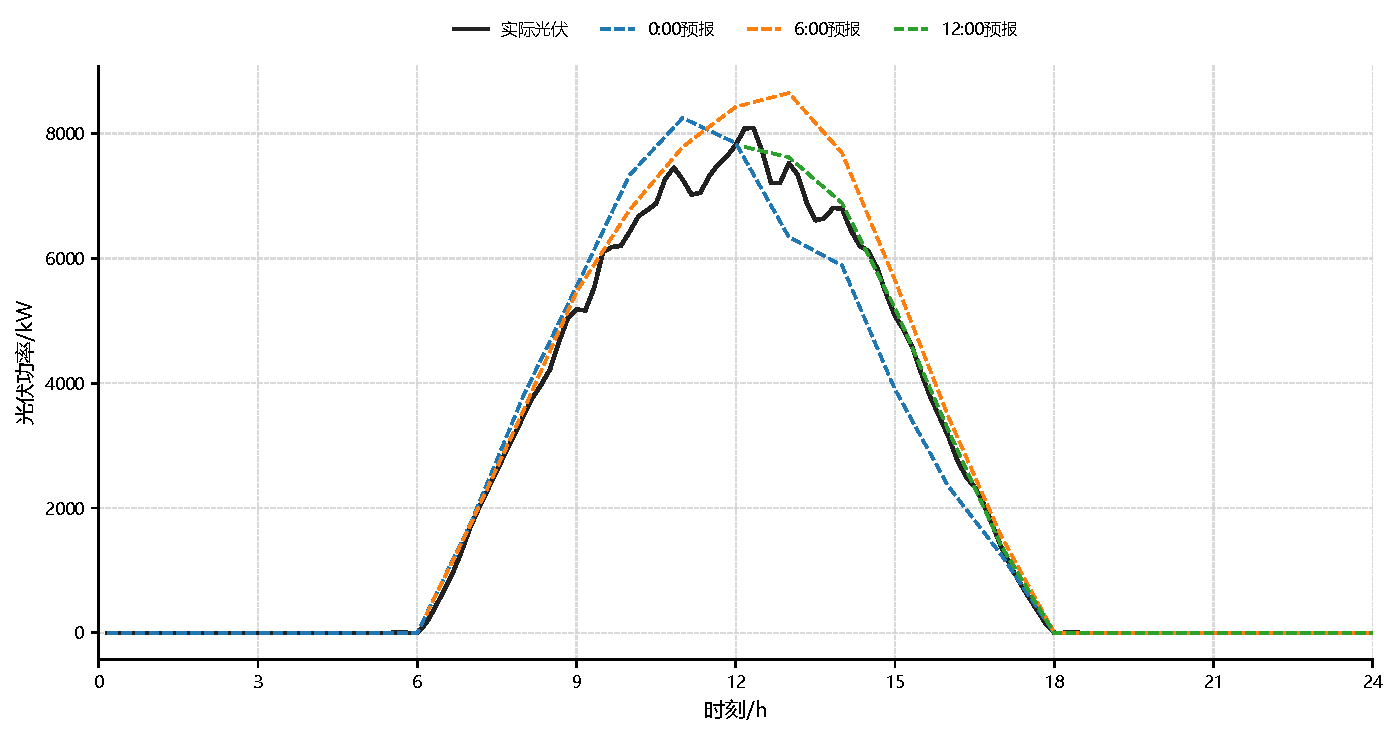
\includegraphics[width=0.72\textwidth]{../figures/问题三/问题三_指定日滚动光伏预报对比.pdf}
  \caption{2025 年 3 月 20 日各发布时点光伏预报与实际光伏对比}
  \label{fig:q3_day_pv}
\end{figure}

该日的滚动调度结果如图~\ref{fig:q3_day_sched} 所示：储能设备在午间低价时段充电、傍晚高价时段放电，实际紧急购电集中在凌晨与傍晚的少数时段。

\begin{figure}[H]
  \centering
  
\includegraphics[width=0.72\textwidth]{../figures/问题三/问题三_指定日滚动调度结果.pdf}
  \caption{2025 年 3 月 20 日滚动调度结果}
  \label{fig:q3_day_sched}
\end{figure}

\FloatBarrier
\section{问题四的模型建立与求解}

\subsection{电价数据的周期结构分析}

设 $\lambda_{d,t}$ 为第 $d$ 天第 $t$ 个 10 分钟时段的实际电价（元/kWh），$d=1,\dots,365$，$t=1,\dots,144$。按星期分类求平均，可得各类星期的典型电价曲线，如图~\ref{fig:q4_periodic} 左图所示。日内分时电价呈稳定的阶梯结构，工作日与周末的价格水平存在明显差异。

将全年电价按时间顺序展开为 10 分钟序列 $x_n$（$n=1,\dots,N$，$N=365\times144$），样本自相关函数为

\begin{equation}
  \widehat\rho(k) = \frac{\displaystyle\sum_{n=k+1}^{N}(x_n-\bar x)(x_{n-k}-\bar x)}{\displaystyle\sum_{n=1}^{N}(x_n-\bar x)^2},
  \label{eq:q4_acf}
\end{equation}

式中：$x_n$ 为第 $n$ 个 10 分钟时段的电价（元/kWh）；$\bar x$ 为序列均值；$k$ 为滞后阶数。一天包含 144 个 10 分钟时段，因此第 $h$ 个整日滞后的自相关系数即 $\widehat\rho(144h)$。计算结果如图~\ref{fig:q4_periodic} 右图所示：第 1、7 个整日滞后分别为 0.9299 与 0.9576，第 14、21、28 个整日滞后分别为 0.9260、0.8947 与 0.8634，均明显高于其相邻的非整周滞后，形成整周局部峰值。据此，把过去 4 个同星期、同时刻的价格作为 0:00 全天预测的输入变量。

\begin{figure}[H]
  \centering
  
\includegraphics[width=0.485\textwidth]{../figures/问题四/问题四_典型星期电价曲线.pdf}\hfill
  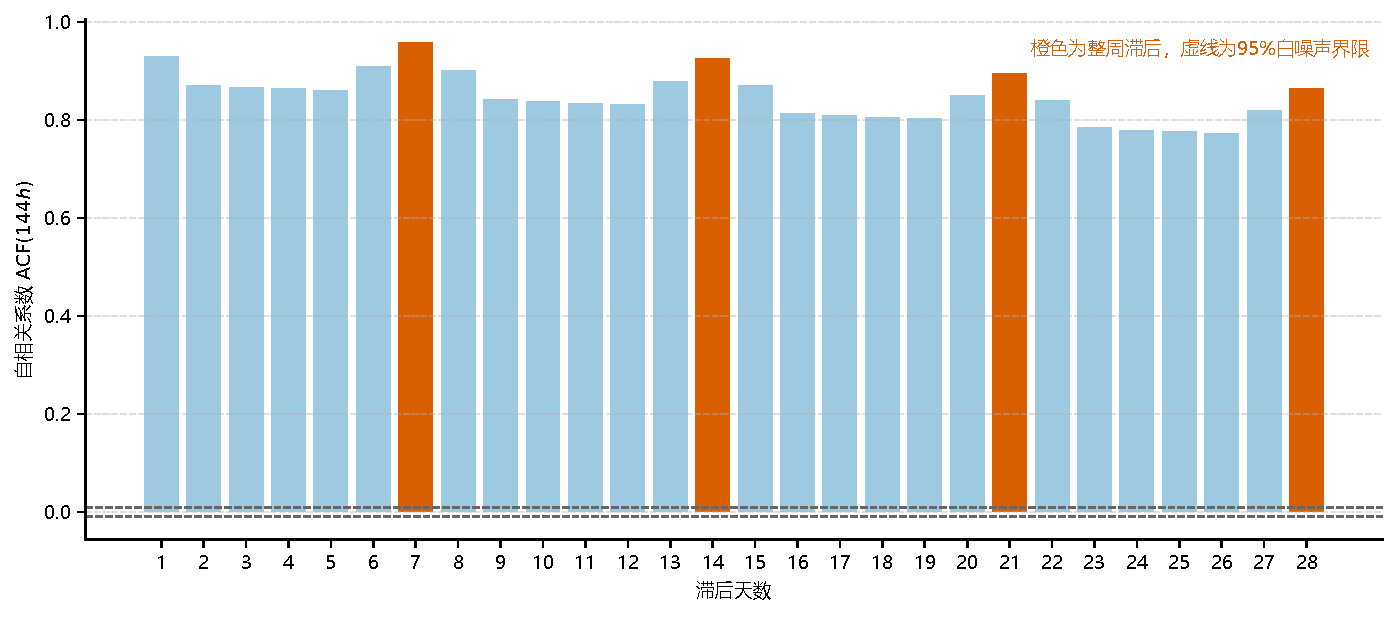
\includegraphics[width=0.485\textwidth]{../figures/问题四/问题四_ACF自相关.pdf}
  \caption{电价周期结构（左：星期一至星期日的典型电价曲线；右：整日滞后自相关函数）}
  \label{fig:q4_periodic}
\end{figure}

\subsection{0:00 固定指数周期电价预测模型}

对计划日 $d$ 的时段 $t$，使用最近至多 4 个同星期、同时刻的价格，即 $\lambda_{d-7k,t}$（$k=1,\dots,K_d$）。可用历史周数为 $K_d=\min\{4,\lfloor (d-1)/7\rfloor\}$，固定指数权重为

\begin{equation}
  w_{d,k} = \frac{\rho^{\,k-1}}{\sum_{j=1}^{K_d}\rho^{\,j-1}}, \qquad \rho = 0.8,
  \label{eq:q4_weight}
\end{equation}

式中：$w_{d,k}$ 为前第 $k$ 个同星期价格的权重；$\rho$ 为衰减系数，取 0.8，使越近的周权重越大。0:00 的电价预测为

\begin{equation}
  \widehat\lambda_{d,t}^{(0)} = \max\left\{\sum_{k=1}^{K_d} w_{d,k}\,\lambda_{d-7k,t},\ 0\right\},
  \label{eq:q4_pred0}
\end{equation}

式中：$\widehat\lambda_{d,t}^{(0)}$ 为计划日 $d$、时段 $t$ 的 0:00 电价预测值（元/kWh）；上标 $(0)$ 表示该预测在 0:00 生成；$\max\{\cdot,0\}$ 用于保证预测价格非负。当 4 周历史全部可用时，归一化权重为 $(w_1,w_2,w_3,w_4) = (0.3388,\ 0.2710,\ 0.2168,\ 0.1734)$。

样本外预测的平均绝对误差为 0.0467 元/kWh，均方根误差为 0.0665 元/kWh，WAPE（按式~\eqref{eq:wape} 计算）为 6.17\%，日内 Spearman 秩相关系数为 0.9526；前 20\% 高价时段识别率为 89.30\%，最高价时刻误差为 119.6 min。上一日同期、上一周同期和最近 4 周简单平均三个对照模型的平均绝对误差依次为 0.0843、0.0472、0.0489 元/kWh，对应秩相关系数为 0.9380、0.9460、0.9517。相较最优对照（上一周同期），四周指数加权模型使平均绝对误差降低 0.91\%，WAPE 由 6.22\% 降至 6.17\%，日内排序相关系数由 0.9460 提升至 0.9526，故用于后续储能调度；各模型误差对比如图~\ref{fig:q4_pred_err} 所示。

\begin{figure}[H]
  \centering
  
\includegraphics[width=0.72\textwidth]{../figures/问题四/问题四_电价预测模型误差对比.pdf}
  \caption{0:00 电价预测模型的误差对比}
  \label{fig:q4_pred_err}
\end{figure}

\subsection{日内因果门控的残差更新}

当天价格相对 0:00 周期基线的残差为 $e_{d,t} = \lambda_{d,t} - \widehat\lambda_{d,t}^{(0)}$。在 6:00、12:00、18:00 三个时点，模型可以使用截至决策时刻已经发生的价格残差。取滞后集合

\begin{equation}
  \mathcal J = \{1,2,3,6,12,18,36,72,144\},
  \label{eq:q4_lags}
\end{equation}

式中：$\mathcal J$ 中各元素为该时刻之前第若干个 10 分钟时段，分别对应 10 分钟至 1 天的时间尺度。建立残差自回归模型

\begin{equation}
  e_n = \beta_0 + \sum_{\ell\in\mathcal J}\beta_\ell\, e_{n-\ell} + \varepsilon_n,
  \label{eq:q4_ar}
\end{equation}

式中：$e_n$ 为第 $n$ 个时段的电价残差（元/kWh）；$\beta_0$ 为截距，$\beta_\ell$ 为各滞后阶的回归系数；$\varepsilon_n$ 为残差项。参数通过岭回归估计\cite{ref7}：

\begin{equation}
  \widehat{\boldsymbol\beta} = \arg\min_{\boldsymbol\beta}\left\{\sum_n \left(e_n-\beta_0-\mathbf x_n^{\mathsf T}\boldsymbol\beta\right)^2 + \alpha\|\boldsymbol\beta\|_2^2\right\},
  \label{eq:q4_ridge}
\end{equation}

式中：$\mathbf x_n$ 为由滞后残差构成的解释向量；$\alpha$ 为正则化参数，从 $\{0.1,1,10,20,50,100\}$ 中通过扩展窗口时间序列验证选取；参数只使用当前月份以前的数据拟合，月内固定，避免逐日重复估计带来的不稳定。

残差更新并非在所有月份都优于周期基线。为此在每月开始前，用最近 7 个可验证历史日比较残差模型与周期基线的 MAE，仅当残差模型更优时该月在该时点启用更新，即

\begin{equation}
  \widehat\lambda_{d,t}^{(\tau)} = \max\left\{\widehat\lambda_{d,t}^{(0)} + I_{d,\tau}\,\widehat e_{d,t}^{(\tau)},\ 0\right\}, \qquad t > \tau,
  \label{eq:q4_gated}
\end{equation}

式中：$\widehat\lambda_{d,t}^{(\tau)}$ 为时点 $\tau$ 更新后的电价预测（元/kWh）；$\widehat e_{d,t}^{(\tau)}$ 为残差模型的预测值；$I_{d,\tau}\in\{0,1\}$ 为门控变量，完全由历史验证结果决定，不依赖当天未来信息。各时点的启用天数与精度改善如表 12 所示。

\threelinetable{表 12\quad 日内门控残差更新的效果}{l r r r}{%
  \textbf{更新时点} & \textbf{启用更新天数} & \textbf{周期基线 MAE} & \textbf{门控更新 MAE（相对改善）}%
}{%
  6:00  & 215 & 0.0518 & 0.0487（5.97\%） \\
  12:00 & 245 & 0.0501 & 0.0457（8.80\%） \\
  18:00 & 93  & 0.0457 & 0.0455（0.35\%） \\
}

表中 MAE 的单位为元/kWh；其统计范围为各时点之后的剩余时域，并在全部 334 天上计算：启用更新的日期使用残差修正后的预测，未启用的日期保持 0:00 周期基线。6:00 与 12:00 的更新明显改善了剩余时域的价格预测，18:00 因剩余时域较短、可用的当天残差信息有限，边际改善很小。

\subsection{三类残差的联合场景生成}

电价预测误差与负荷、光伏预测误差存在相关性，若分别独立抽样可能生成``高负荷与低价格''等缺乏历史依据的场景。因此对每个历史日 $r$ 保存严格样本外的三类残差

\begin{equation}
  \left(e^L_r(t),\ e^P_r(t),\ e^{\lambda,\tau}_r(t)\right),
  \qquad
  e^{\lambda,\tau}_r(t) = \lambda_r(t) - \widehat\lambda^{(\tau)}_{r,t},
  \label{eq:q4_joint_res}
\end{equation}

式中：$e^{\lambda,\tau}_r(t)$ 为历史日期 $r$ 在时点 $\tau$ 的电价预测残差（元/kWh）。三类残差按同一个历史日期联合抽取，每个决策模型抽取 30 个历史日，重复抽中的日期按频数合并并赋予相应场景概率，从而在不改变经验分布的前提下降低混合整数规划的规模。价格场景为

\begin{equation}
  \lambda^{(\tau)}_{d,s}(t) = \max\left\{\widehat\lambda^{(\tau)}_{d,t} + e^{\lambda,\tau}_{r_s}(t),\ 0\right\},
  \label{eq:q4_price_scenario}
\end{equation}

式中：$\lambda^{(\tau)}_{d,s}(t)$ 为时点 $\tau$、计划日 $d$、场景 $s$、时段 $t$ 的电价场景（元/kWh）；$r_s$ 为本次抽中的历史日期。

\subsection{问题 4-2：单时点计划模型与结果}

问题 4-2 只使用 0:00 的周期电价预测，不引入当天残差更新，其模型结构与问题二一致，同样采用季节余弦终端软区间，只是把固定的日内电价 $\lambda(t)$ 替换为随场景变化的价格。目标函数为

\begin{equation}
  \min\left\{
    \sum_s \pi_s \sum_t\left[\lambda_{d,s}(t)G_d(t) + 5\lambda_{d,s}(t)H_{d,s}(t)\right]
    + \kappa_d\,(R_d + X_d)
  \right\},
  \label{eq:q4_obj2}
\end{equation}

式中：$\lambda_{d,s}(t)$ 为场景电价（元/kWh）；$\kappa_d$ 为终端偏离惩罚系数，其含义与式~\eqref{eq:kappa} 中的 $\kappa$ 相同，只是改用计划日之前已经发生的实际电价分位数逐日构造，同样取 $\kappa_d = 0.9\,Q_{0.90}(\lambda)$，从而不使用未来电价；终端偏离惩罚只用于决策，不计入实际支付费用。场景电量平衡同式~\eqref{eq:q2_balance}，储能状态递推、容量边界与充放电互斥约束同式~\eqref{eq:q2_soc} 与式~\eqref{eq:q2_mutex}，储电量跨日连续传递。问题 4-2 的全年结果如表 13 所示。

{\footnotesize
\threelinetable{表 13\quad 问题 4-2 全年结果}{l r l r}{%
  \textbf{指标} & \textbf{结果} & \textbf{指标} & \textbf{结果}%
}{%
  计划购电量/kWh & 22229426.39 & 正常购电费/元 & 14301863.64 \\
  紧急购电量/kWh & 305254.47 & 紧急购电费/元 & 1227651.14 \\
  富余电量/kWh & 3248071.91 & 实际总费用/元 & 15529514.78 \\
  充电量/kWh & 7089161.18 & 发生紧急购电天数 & 327 \\
  放电量/kWh & 5741741.73 & 平均日末储电量/kWh & 5975.44 \\
  12 月 31 日末储电量/kWh & 6532.02 & & \\
}
}

\subsection{问题 4-3：四时点滚动模型与结果}

问题 4-3 在 0:00 制定全天计划后，于 6:00、12:00、18:00 利用当天已观测价格与附件 3 的最新光伏预报滚动调整剩余时域。设 0:00 原计划购电量为 $G_d(t)$、调整后购电量为 $A_d(t)$，调整量为

\begin{equation}
  A_d(t) - G_d(t) = U_d(t) - V_d(t), \qquad U_d(t),\,V_d(t) \ge 0,
  \label{eq:q4_adjust}
\end{equation}

式中：$U_d(t)$ 与 $V_d(t)$ 分别为相对原计划的上调量与下调量（kWh）。在决策时点 $\tau$ 对剩余时域 $\mathcal T_\tau$ 求解

\begin{equation}
  \min\left\{
    \sum_s \pi_s \sum_{t\in\mathcal T_\tau}\left[1.5\lambda^{(\tau)}_{d,s}(t)U_d(t) - 0.5\lambda^{(\tau)}_{d,s}(t)V_d(t) + 5\lambda^{(\tau)}_{d,s}(t)H_{d,s}(t)\right]
    + \kappa_d\,(R_d^{(\tau)} + X_d^{(\tau)})
  \right\},
  \label{eq:q4_obj3}
\end{equation}

式中：方括号内三项依次为上调加价费、下调抵扣（负值）与紧急购电费（元），系数含义与问题三相同。每次求解至当天 24:00，但只执行到下一个更新时点：0:00 结果执行至 6:00，6:00 结果执行至 12:00，12:00 结果执行至 18:00，18:00 结果执行至 24:00。已执行时段的购电量、充放电量与储电量不得回溯修改，每次优化的初始储电量等于上一已执行时段的实际储电量。

四种策略费用依次为 15778106.07、15553894.38、15397581.11 和 15393286.54 元。正式 4-3 相对仅 0:00 策略节省 384819.53 元（2.44\%），紧急购电量减少 27.73\%；其中 6:00 与 12:00 更新贡献绝大部分收益，18:00 的边际改善很小。按净结算口径，4-3 的计划与调整结算费、紧急购电费分别为 14462432.65 元、930853.89 元；相对 4-2 节省 136228.24 元（0.88\%），表明波动电价下的日内滚动同样有效。

\subsubsection{指定日期的完整结果}

指定日期的购电、储能与紧急购电结果分别见表 14 至表 16。

{\scriptsize
\threelinetable{表 14\quad 问题四 4-2指定日期的购电结果}{l r r r r}{%
  \textbf{时间段} & \textbf{3 月 20 日} & \textbf{6 月 21 日} & \textbf{9 月 23 日} & \textbf{12 月 21 日}%
}{%
  10:00--10:10 & 0.00 & 0.00 & 0.00 & 0.00 \\
12:00--12:10 & 573.58 & 0.00 & 519.74 & 1004.00 \\
14:00--14:10 & 0.00 & 0.00 & 0.00 & 0.00 \\
16:00--16:10 & 486.58 & 234.98 & 561.13 & 863.31 \\
18:00--18:10 & 0.00 & 474.62 & 0.00 & 733.12 \\
20:00--20:10 & 245.31 & 0.00 & 1.68 & 0.00 \\
全天购电量/kWh & 69382.94 & 39149.55 & 72824.93 & 96979.31 \\
全天购电费/元 & 43039.58 & 19453.65 & 47391.27 & 73185.53 \\
}

}

{\tiny
\begin{center}
  {\fontsize{10.5pt}{12.6pt}\heiti\bfseries 表 15\quad 问题四 4-2指定日期的储能结果}\par
  \vspace{0.25em}
  \resizebox{\textwidth}{!}{%
  \begin{tabular}{l r r r r r r r r}
    \toprule
    & \multicolumn{2}{c}{\textbf{3 月 20 日}} & \multicolumn{2}{c}{\textbf{6 月 21 日}} & \multicolumn{2}{c}{\textbf{9 月 23 日}} & \multicolumn{2}{c}{\textbf{12 月 21 日}} \\
    \cmidrule(lr){2-3}\cmidrule(lr){4-5}\cmidrule(lr){6-7}\cmidrule(lr){8-9}
    \textbf{时间段} & \textbf{充电量/kWh} & \textbf{放电量/kWh} & \textbf{充电量/kWh} & \textbf{放电量/kWh} & \textbf{充电量/kWh} & \textbf{放电量/kWh} & \textbf{充电量/kWh} & \textbf{放电量/kWh} \\
    \midrule
    0:00-4:00 & 4574.89 & 0.00 & 0.00 & 1560.22 & 4693.29 & 0.00 & 3710.18 & 0.00 \\
4:00-8:00 & 637.77 & 5964.14 & 865.01 & 2168.11 & 833.33 & 5591.98 & 833.33 & 833.33 \\
8:00-12:00 & 5991.01 & 3192.46 & 6240.88 & 0.00 & 6068.93 & 3048.02 & 5833.33 & 7806.67 \\
12:00-16:00 & 5108.41 & 350.53 & 3277.86 & 0.00 & 4943.03 & 279.69 & 8178.38 & 2709.49 \\
16:00-20:00 & 0.00 & 6644.47 & 0.00 & 5956.18 & 0.00 & 6630.91 & 0.00 & 5605.82 \\
20:00-24:00 & 5957.42 & 1995.53 & 5475.29 & 3428.99 & 4966.73 & 2009.09 & 6217.40 & 3034.18 \\
0:00 储电量/kWh & \multicolumn{2}{c}{6682.60} & \multicolumn{2}{c}{5597.21} & \multicolumn{2}{c}{5826.04} & \multicolumn{2}{c}{6710.84} \\
24:00 储电量/kWh & \multicolumn{2}{c}{6561.68} & \multicolumn{2}{c}{5299.79} & \multicolumn{2}{c}{5670.05} & \multicolumn{2}{c}{6795.66} \\
    \bottomrule
  \end{tabular}%
  }
\end{center}
}

{\scriptsize
\threelinetable{表 16\quad 问题四 4-2指定日期的紧急购电结果}{l r l r l r l r}{%
  \textbf{3 月 20 日 时段} & \textbf{购电量/kWh} & \textbf{6 月 21 日 时段} & \textbf{购电量/kWh} & \textbf{9 月 23 日 时段} & \textbf{购电量/kWh} & \textbf{12 月 21 日 时段} & \textbf{购电量/kWh}%
}{%
  0:30-0:40 & 24.54 & 0:30-0:40 & 15.83 & 5:00-5:20 & 15.93 & 1:10-1:30 & 27.03 \\
1:20-1:40 & 44.22 & 1:30-1:50 & 22.00 & 5:50-6:00 & 2.67 & 1:40-2:00 & 18.05 \\
2:40-2:50 & 2.61 & 3:00-3:40 & 28.30 & 6:20-6:40 & 8.42 & 2:10-2:30 & 33.52 \\
3:10-3:40 & 70.70 & 6:10-6:20 & 5.12 & 7:00-7:10 & 6.32 & 3:10-3:30 & 77.84 \\
11:10-11:30 & 57.69 & 19:10-19:20 & 32.59 & 9:50-10:00 & 4.54 & 3:40-4:30 & 137.21 \\
12:40-13:00 & 97.74 &  &  & 10:10-10:20 & 13.11 & 5:10-5:30 & 21.52 \\
15:00-15:10 & 5.33 &  &  & 14:30-15:30 & 282.81 & 5:50-6:50 & 166.55 \\
15:20-16:30 & 346.56 &  &  & 16:00-16:20 & 45.40 & 7:00-7:10 & 0.68 \\
16:40-17:00 & 26.91 &  &  & 16:40-16:50 & 8.73 & 7:20-7:30 & 14.48 \\
17:10-17:30 & 11.28 &  &  & 18:40-18:50 & 9.53 & 8:00-8:10 & 6.34 \\
18:50-19:20 & 92.03 &  &  & 20:20-20:40 & 28.31 & 10:30-11:50 & 451.31 \\
20:10-20:30 & 17.74 &  &  & 21:00-21:10 & 43.75 & 13:00-13:20 & 34.61 \\
21:30-21:50 & 19.92 &  &  & 22:30-22:40 & 15.59 & 17:30-17:40 & 10.73 \\
23:40-0:00+1 & 53.62 &  &  &  &  & 18:50-19:10 & 6.86 \\
 &  &  &  &  &  & 19:50-20:10 & 56.60 \\
 &  &  &  &  &  & 22:00-22:10 & 4.07 \\
 &  &  &  &  &  & 23:00-23:10 & 9.65 \\
 &  &  &  &  &  & 23:50-0:00+1 & 7.19 \\
}
}

\subsubsection{指定日期的完整结果}

指定日期的购电、储能与紧急购电结果分别见表 17 至表 19。

{\scriptsize
\threelinetable{表 17\quad 问题四 4-3指定日期的购电结果}{l r r r r}{%
  \textbf{时间段} & \textbf{3 月 20 日} & \textbf{6 月 21 日} & \textbf{9 月 23 日} & \textbf{12 月 21 日}%
}{%
  10:00--10:10 & 0.00 / 0.00 & 0.00 / 0.00 & 0.00 / 0.00 & 0.00 / 0.00 \\
12:00--12:10 & 658.00 / 567.69 & 0.00 / 0.00 & 513.04 / 444.43 & 995.84 / 966.61 \\
14:00--14:10 & 64.20 / 0.00 & 0.00 / 0.00 & 0.00 / 0.00 & 0.00 / 0.00 \\
16:00--16:10 & 659.13 / 541.66 & 233.76 / 187.28 & 603.11 / 603.11 & 872.14 / 872.14 \\
18:00--18:10 & 0.00 / 0.00 & 514.48 / 514.48 & 6.40 / 6.40 & 725.44 / 725.44 \\
20:00--20:10 & 216.35 / 216.35 & 0.00 / 0.00 & 8.21 / 32.69 & 0.00 / 0.00 \\
全天购电量/kWh（计划 / 调整后） & 74034.74 / 69070.05 & 38182.76 / 37819.52 & 76301.19 / 74112.62 & 96829.39 / 96192.18 \\
全天购电费/元（计划 / 调整后） & 46301.64 / 44560.42 & 19316.49 / 19209.60 & 50120.63 / 49802.86 & 72877.93 / 72637.91 \\
}
单元格依次为 0:00 计划值与最终调整后执行值。
}

{\tiny
\begin{center}
  {\fontsize{10.5pt}{12.6pt}\heiti\bfseries 表 18\quad 问题四 4-3指定日期的储能结果}\par
  \vspace{0.25em}
  \resizebox{\textwidth}{!}{%
  \begin{tabular}{l r r r r r r r r}
    \toprule
    & \multicolumn{2}{c}{\textbf{3 月 20 日}} & \multicolumn{2}{c}{\textbf{6 月 21 日}} & \multicolumn{2}{c}{\textbf{9 月 23 日}} & \multicolumn{2}{c}{\textbf{12 月 21 日}} \\
    \cmidrule(lr){2-3}\cmidrule(lr){4-5}\cmidrule(lr){6-7}\cmidrule(lr){8-9}
    \textbf{时间段} & \textbf{充电量/kWh} & \textbf{放电量/kWh} & \textbf{充电量/kWh} & \textbf{放电量/kWh} & \textbf{充电量/kWh} & \textbf{放电量/kWh} & \textbf{充电量/kWh} & \textbf{放电量/kWh} \\
    \midrule
    0:00-4:00 & 4166.67 & 0.00 & 0.00 & 2771.92 & 4166.67 & 0.00 & 4166.67 & 0.00 \\
4:00-8:00 & 1217.06 & 6225.18 & 833.33 & 2101.23 & 1160.75 & 6061.42 & 446.32 & 871.02 \\
8:00-12:00 & 5305.69 & 2470.84 & 5913.23 & 0.00 & 5935.89 & 2430.50 & 5833.33 & 7448.16 \\
12:00-16:00 & 5815.79 & 366.84 & 4753.44 & 0.00 & 5463.76 & 783.26 & 7808.70 & 2736.31 \\
16:00-20:00 & 7.34 & 5901.89 & 6.30 & 5931.75 & 61.02 & 6139.65 & 16.87 & 5642.04 \\
20:00-24:00 & 6120.50 & 2745.68 & 6109.96 & 3459.73 & 4951.78 & 2513.93 & 6177.31 & 3014.38 \\
0:00 储电量/kWh & \multicolumn{2}{c}{6015.16} & \multicolumn{2}{c}{5864.61} & \multicolumn{2}{c}{6005.33} & \multicolumn{2}{c}{6648.31} \\
24:00 储电量/kWh & \multicolumn{2}{c}{6706.64} & \multicolumn{2}{c}{5869.65} & \multicolumn{2}{c}{5650.36} & \multicolumn{2}{c}{6750.47} \\
    \bottomrule
  \end{tabular}%
  }
\end{center}
}

{\scriptsize
\threelinetable{表 19\quad 问题四 4-3指定日期的紧急购电结果}{l r l r l r l r}{%
  \textbf{3 月 20 日 时段} & \textbf{购电量/kWh} & \textbf{6 月 21 日 时段} & \textbf{购电量/kWh} & \textbf{9 月 23 日 时段} & \textbf{购电量/kWh} & \textbf{12 月 21 日 时段} & \textbf{购电量/kWh}%
}{%
  0:30-0:40 & 26.81 & 0:30-0:40 & 2.65 & 5:10-5:20 & 17.28 & 0:10-0:30 & 3.85 \\
1:20-1:50 & 52.28 & 1:30-1:40 & 10.42 & 7:50-8:00 & 2.39 & 1:10-1:30 & 9.33 \\
2:40-3:00 & 8.22 & 2:20-2:30 & 0.22 & 21:00-21:20 & 39.99 & 1:40-1:50 & 6.75 \\
3:20-3:40 & 41.91 & 3:00-3:40 & 42.49 &  &  & 2:10-2:30 & 10.78 \\
5:10-5:20 & 4.25 & 19:10-19:20 & 10.45 &  &  & 3:10-3:30 & 67.44 \\
8:10-9:30 & 256.67 &  &  &  &  & 3:40-4:10 & 97.87 \\
9:50-10:10 & 75.55 &  &  &  &  & 4:20-4:30 & 0.23 \\
11:10-12:10 & 193.22 &  &  &  &  & 5:10-5:30 & 13.05 \\
12:40-13:40 & 263.99 &  &  &  &  & 5:50-6:40 & 64.34 \\
14:10-14:20 & 3.15 &  &  &  &  & 7:10-7:20 & 2.24 \\
16:10-16:30 & 26.18 &  &  &  &  & 8:00-8:10 & 3.15 \\
18:10-18:20 & 1.82 &  &  &  &  & 8:50-9:10 & 30.18 \\
18:50-19:20 & 94.52 &  &  &  &  & 9:40-10:10 & 56.21 \\
20:10-20:30 & 27.51 &  &  &  &  & 10:30-12:10 & 467.75 \\
21:30-21:50 & 19.17 &  &  &  &  & 12:50-13:20 & 18.50 \\
23:40-0:00+1 & 38.22 &  &  &  &  & 17:30-17:40 & 8.16 \\
 &  &  &  &  &  & 18:50-19:10 & 10.03 \\
 &  &  &  &  &  & 19:50-20:10 & 59.27 \\
 &  &  &  &  &  & 23:00-23:10 & 6.35 \\
 &  &  &  &  &  & 23:40-0:00+1 & 20.04 \\
}
}


2025 年 3 月 20 日的价格预测、滚动购电量与储电量轨迹如图~\ref{fig:q4_day} 所示。

\begin{figure}[H]
  \centering
  
\includegraphics[width=0.72\textwidth]{../figures/问题四/问题四_指定日价格预测与滚动调度.pdf}
  \caption{2025 年 3 月 20 日价格预测与滚动调度结果}
  \label{fig:q4_day}
\end{figure}

% 价格完全信息下界已移入第八章的方案对比，避免与敏感性分析重复。
\endinput
\subsection{价格完全信息下界}

为量化电价预测误差造成的经济损失，保持负荷与光伏场景的信息结构与现实策略一致，只把未来价格场景替换为当天的实际价格：

\begin{equation}
  \lambda_{d,s}(t) = \lambda^{\mathrm{act}}_d(t), \qquad F^{\mathrm{PI}}_{4\text{-}j}, \quad j\in\{2,3\},
  \label{eq:q4_PI}
\end{equation}

式中：$\lambda^{\mathrm{act}}_d(t)$ 为当天的实际电价（元/kWh）；$F^{\mathrm{PI}}_{4\text{-}j}$ 为价格完全信息下问题 $4\text{-}j$ 的最优费用（元）。价格信息损失定义为 $\Delta F^{\lambda}_{4\text{-}j} = F^{\mathrm{reality}}_{4\text{-}j} - F^{\mathrm{PI}}_{4\text{-}j}$，式中 $F^{\mathrm{reality}}_{4\text{-}j}$ 为现实策略的实际总费用。计算结果为：问题 4-2 的完全信息下界为 15386096.19 元，价格信息损失 143418.60 元，占下界的 0.93\%；问题 4-3 的完全信息下界为 15236867.28 元，价格信息损失 156419.25 元，占下界的 1.03\%。由于完全信息模型只放开未来实际价格，负荷与光伏仍保持现实的信息结构，该差额可解释为纯粹的价格预测误差造成的经济损失，其相对下界的差距在 1\% 左右，说明本文的周期电价预测已经捕获了绝大部分可用于储能套利的价格信息。反之，若把附件 4 的当天实际电价直接代入日前决策，得到的正是该完全信息解，它只能作为理论下界，不能当作可实施的策略。

需要说明的是，问题四使用附件 4 的实时波动电价，而问题二使用附件 1 的固定日内电价，两者的价格结构与结算口径不同，全年费用不可直接比较。附件 4 的全年平均电价与附件 1 一致（均为 0.7662 元/kWh），但其日内峰谷极差明显更大；即使给定完全信息，波动电价下的最优调度费用仍高于固定电价情形，说明电价波动本身会提高储能的调度难度与购电成本。

\FloatBarrier
\section{敏感性分析}

为检验结论的稳健性，本文将已有的方案对照与新增的参数扫描分开讨论。前者复用前文各问题的正式结果，后者仅针对问题四 4-3 的四时点滚动模型进行年度回测。

\subsection{方案对比}

表 20 汇总终端机制、滚动更新和价格信息结构的对照结果。问题二中，季节余弦终端基准叠加因果风险微调后，年度费用较固定 6000~kWh 终端基线降低 2836.86 元（0.02\%）。该变化较小，说明终端机制的主要作用是避免跨日储能透支，而非追求单日费用的显著下降。

问题三和问题四 4-3 中，全部四时点滚动相对仅 0:00 决策分别节省 351055.72 元（2.36\%）和 384819.53 元（2.44\%）。两种价格口径下的降幅接近，且 6:00 与 12:00 更新贡献绝大部分收益，故日内滚动的经济价值主要来自对负荷、光伏不确定性的及时修正。

价格完全信息下界仅将未来电价替换为实际值，负荷与光伏的信息结构、储能约束及滚动时点均保持不变；因此它衡量的是价格预测误差的经济影响，而不是所有预测变量均准确时的全局理论最优。问题 4-2 与 4-3 相对该下界的差距分别为 0.93\% 和 1.03\%，表明现有周期预测和日内门控更新已捕获大部分可用于套利的价格信息。

\Needspace{8\baselineskip}
{\footnotesize
\threelinetable{表 20\quad 模型方案与价格信息对照}{l r r r r}{%
  \textbf{对比对象} & \textbf{基准费用/元} & \textbf{对照费用或下界/元} & \textbf{费用变化/元} & \textbf{相对变化}\\
}{%
  问题二：固定终端 $\rightarrow$ 季节余弦 + 风险微调 & 14640006.24 & 14637169.37 & $-2836.86$ & $-0.02\%$\\
  问题三：仅 0:00 $\rightarrow$ 全部四时点滚动 & 14861411.71 & 14510355.99 & $-351055.72$ & $-2.36\%$\\
  问题四 4-3：仅 0:00 $\rightarrow$ 全部四时点滚动 & 15778106.07 & 15393286.54 & $-384819.53$ & $-2.44\%$\\
  问题四 4-2：现实预测 $\rightarrow$ 价格完全信息下界 & 15529514.78 & 15386096.19 & $-143418.60$ & $-0.93\%$\\
  问题四 4-3：现实预测 $\rightarrow$ 价格完全信息下界 & 15393286.54 & 15236867.28 & $-156419.25$ & $-1.03\%$\\
}
}

\subsection{参数对比}

以问题四 4-3 的正式模型为基准，取 $\rho=0.80$、场景数 $S=100$、终端软区间半宽 $h=1000$~kWh；单次仅改变一个参数，其余规则保持不变。图~\ref{fig:q4_sensitivity_cost} 与表~21 给出扫描结果；场景数各水平采用 5 个共同随机种子，误差棒为年度费用标准差。

$\rho$ 的三个离散点费用差异不超过 $0.23\%$；$S$ 从 50 至 200 时，费用由 $+0.17\%$ 变为 $-0.09\%$、单日求解时间由 1.30~s 增至 1.97~s，故保留 $S=100$；$h=500$--$1500$~kWh 时费用变化不超过 $0.02\%$。

\begin{figure}[H]
  \centering
  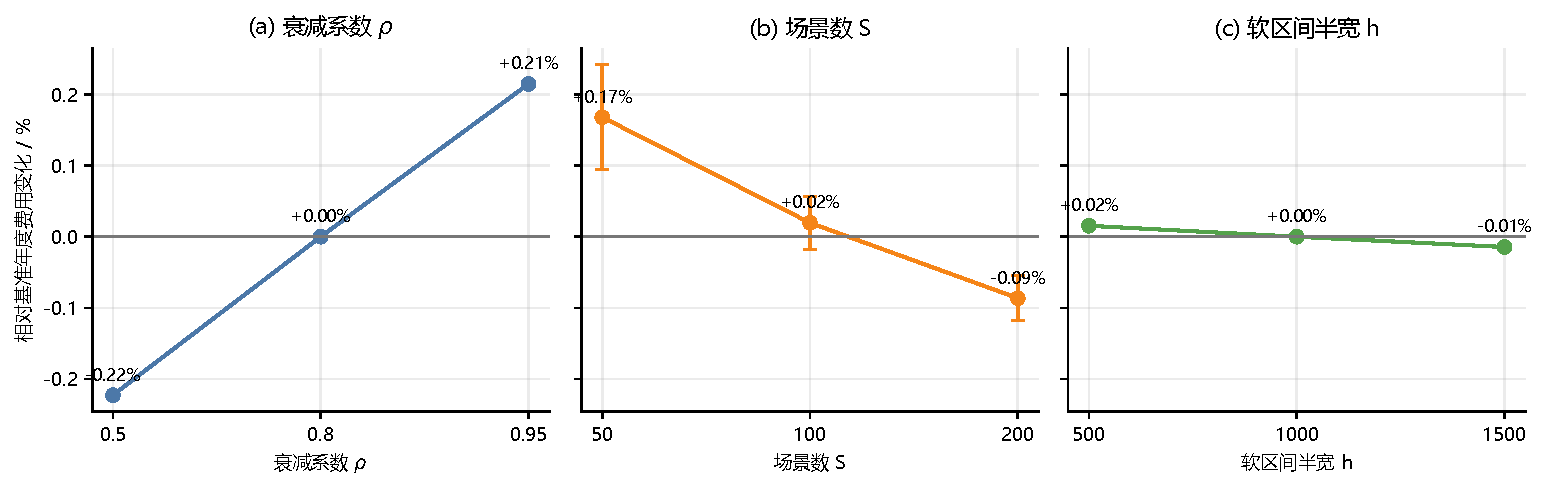
\includegraphics[width=0.60\textwidth]{../figures/问题四/问题四_4_3年度费用参数灵敏度.pdf}
  \caption{问题四 4-3 年度费用参数灵敏度}
  \label{fig:q4_sensitivity_cost}
\end{figure}

{\scriptsize\renewcommand{\arraystretch}{0.82}
\threelinetable{表 21\quad 问题四 4-3 单参数扫描结果}{l c c l}{%
  \textbf{参数} & \textbf{试验值} & \textbf{年度费用相对基准变化} & \textbf{说明}\\
}{%
  $\rho$ & 0.50 / 0.80 / 0.95 & $-0.22\%$ / $0.00\%$ / $+0.21\%$ & 三个点的差异均小于 0.23\%\\
  $S$ & 50 / 100 / 200 & $+0.17\%$ / $+0.02\%$ / $-0.09\%$ & 5 个种子均值，标准差为 0.07\% / 0.04\% / 0.03\%\\
  $h$/kWh & 500 / 1000 / 1500 & $+0.02\%$ / $0.00\%$ / $-0.01\%$ & 费用影响可忽略\\
}
}

综上，参数扰动不改变主要结论，日内滚动在两类电价口径下均带来约 2.4\% 的稳定费用节省。

\section{模型总结}

本文围绕微网在不同信息条件下的购电与储能调度问题，构建了由日前计划、预测场景与日内修正逐层递进的统一框架。问题一在电价、负荷和光伏完全已知时，以电力平衡、储能状态递推和充放电互斥为约束，给出确定性优化基准；问题二将信息边界限定在每日 0:00，以周期加权预测和整日联合残差场景刻画负荷、光伏的不确定性，并以季节余弦终端软区间维持跨日储能价值；问题三利用官方光伏预报在 6:00、12:00、18:00 对剩余时域滚动优化；问题四进一步处理实时波动电价，以周期预测为基线、以因果门控残差模型完成日内更新。四个问题的约束内核一致，因而不同信息结构下的结果具有可比性。

结果表明，储能能够通过低价充电、高价放电和吸收光伏富余电量有效降低购电成本：完全信息的确定性调度相对无储能基准节省 26.90\%，并消除弃光。面对负荷、光伏及电价的不确定性，严格按可得信息制定的日前与滚动策略仍保持稳定收益。问题三的四时点策略较仅 0:00 决策节省 2.36\%，问题四 4-3 的对应降幅为 2.44\%，且两类情形均显示 6:00、12:00 更新最具经济价值。价格完全信息下界与现实策略的费用差距约为 1\%，说明周期预测结合门控更新已提取了大部分可用于储能套利的价格信息。

本模型的优点在于：预测、残差归档、场景抽样和更新决策均遵循严格的时间信息边界；储能容量、功率、效率及充放电互斥约束保证策略可执行；以实际数据回放结算，使费用结论可复核、可复现。模型尚未显式计入电池退化成本、向外部电网售电机制及极端天气导致的预测分布突变，且终端软区间仍为经验性跨日备用安排。后续可引入寿命损耗与碳排放等多目标成本，结合更长预测窗口和鲁棒或分布鲁棒优化，进一步提升极端场景下的经济性与安全裕度。


% 参考文献紧接正文排版，不另起新页
\section*{AI 工具使用声明}
\addcontentsline{toc}{section}{AI 工具使用声明}
本参赛队在竞赛过程中使用了 AI 工具，主要用于语言润色、代码调试、论文排版与结构优化等，详细使用情况见支撑材料。
\vspace{0.5em}
\referencescn
\newpage
\appendixcn

\end{document}
